\chapter{Quantum algorithms}
\thispagestyle{chapterBeginStyle}
\label{chapter3}

In this chapter we are going to present three main applications of quantum computers: quantum search, algorithms based on quantum Fourier transform and simulations of Hamiltonians. We will show the implementation of Grover's and Shors's algorithms as examples from the first two categories. Finally, we will show simple quantum circuit (although not created out of elementary gates), which can simulate behavior of a simple physical system.

\section{Quantum search algorithm}\label{quantum_search_algorithm}

Let's consider a simple scenario, in which we would like to store 2-bit numbers in a classic database. To achieve this goal, we would need separate bits for each saved number. For example, if we would like to store all possible 2-bit numbers 00, 01, 10, 11, we would need 8 bits in total. At the same time, we could store all of the states $|00\rangle$, $|01\rangle$, $|10\rangle$, $|11\rangle$ on only 2 qubits. We would just assign the same probability to each of these states (obtain uniform superposition):

\[ |s\rangle = \frac{1}{2}|00\rangle + \frac{1}{2}|01\rangle + \frac{1}{2}|10\rangle + \frac{1}{2}|11\rangle\]

(during the measurement we get the square of the factor next to the state, to which the system collapses, so we have a $\frac{1}{4}$ probability of obtaining each of the elementary states). The initial state for our algorithm will be exactly this uniform superposition: $|\psi_0\rangle = |s\rangle$. It can be obtained by applying Hadamard gate to each qubit, which is denoted as $H^{\otimes n}$ (where \textit{n} is a number of qubits).

Now let's say, that we are searching for a number $|w\rangle$ in our quantum database. In that case, we can represent our superposition as a vector in space spanned by vectors $|w\rangle$ and $|s'\rangle$ (the latter one is just an orthonormal vector to the vector $|w\rangle$).

\begin{figure}[ht]
\centering
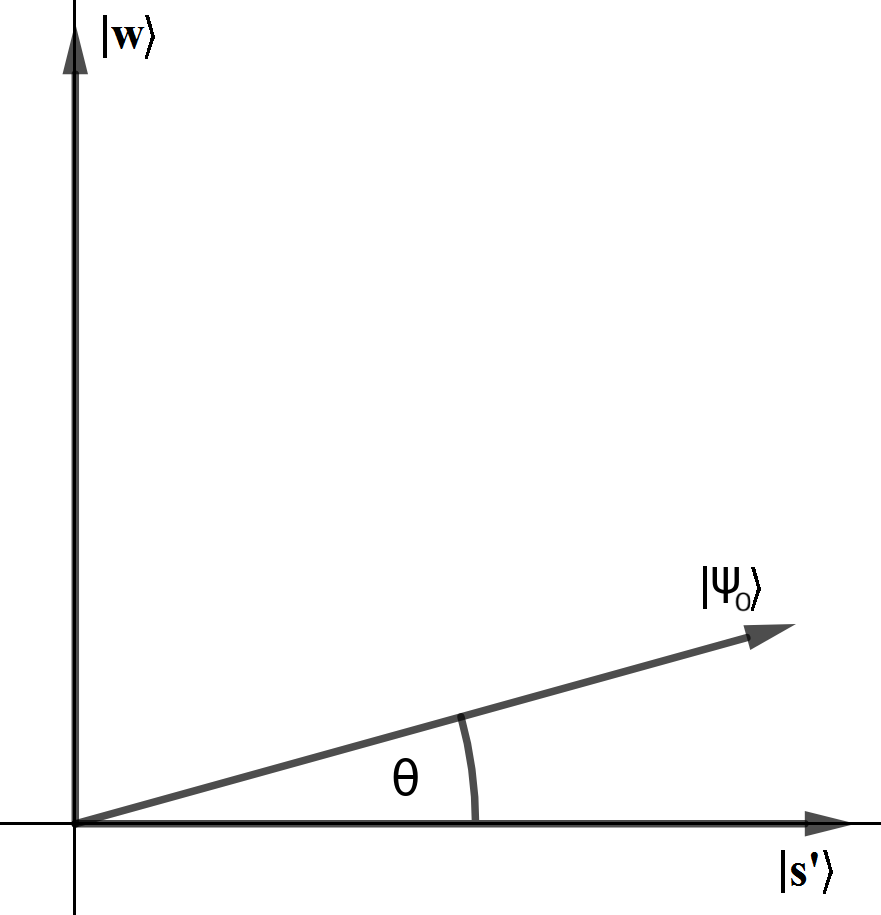
\includegraphics[scale=0.25]{grover_1}
\caption{Representation of the uniform superposition of stored numbers as a vector.}
\end{figure}

As mentioned earlier $|\psi_0\rangle$ is a uniform superposition, so $|w\rangle$ vector is one of its components. Due to this, $|\psi_0\rangle$ cannot be perpendicular to the $|w\rangle$ vector, but it also has to be above the $|s'\rangle$ (because it has to be between these two basis vectors). The initial state $|\psi_0\rangle$ can be also shown on a bar diagram:

\begin{figure}[ht]
\centering
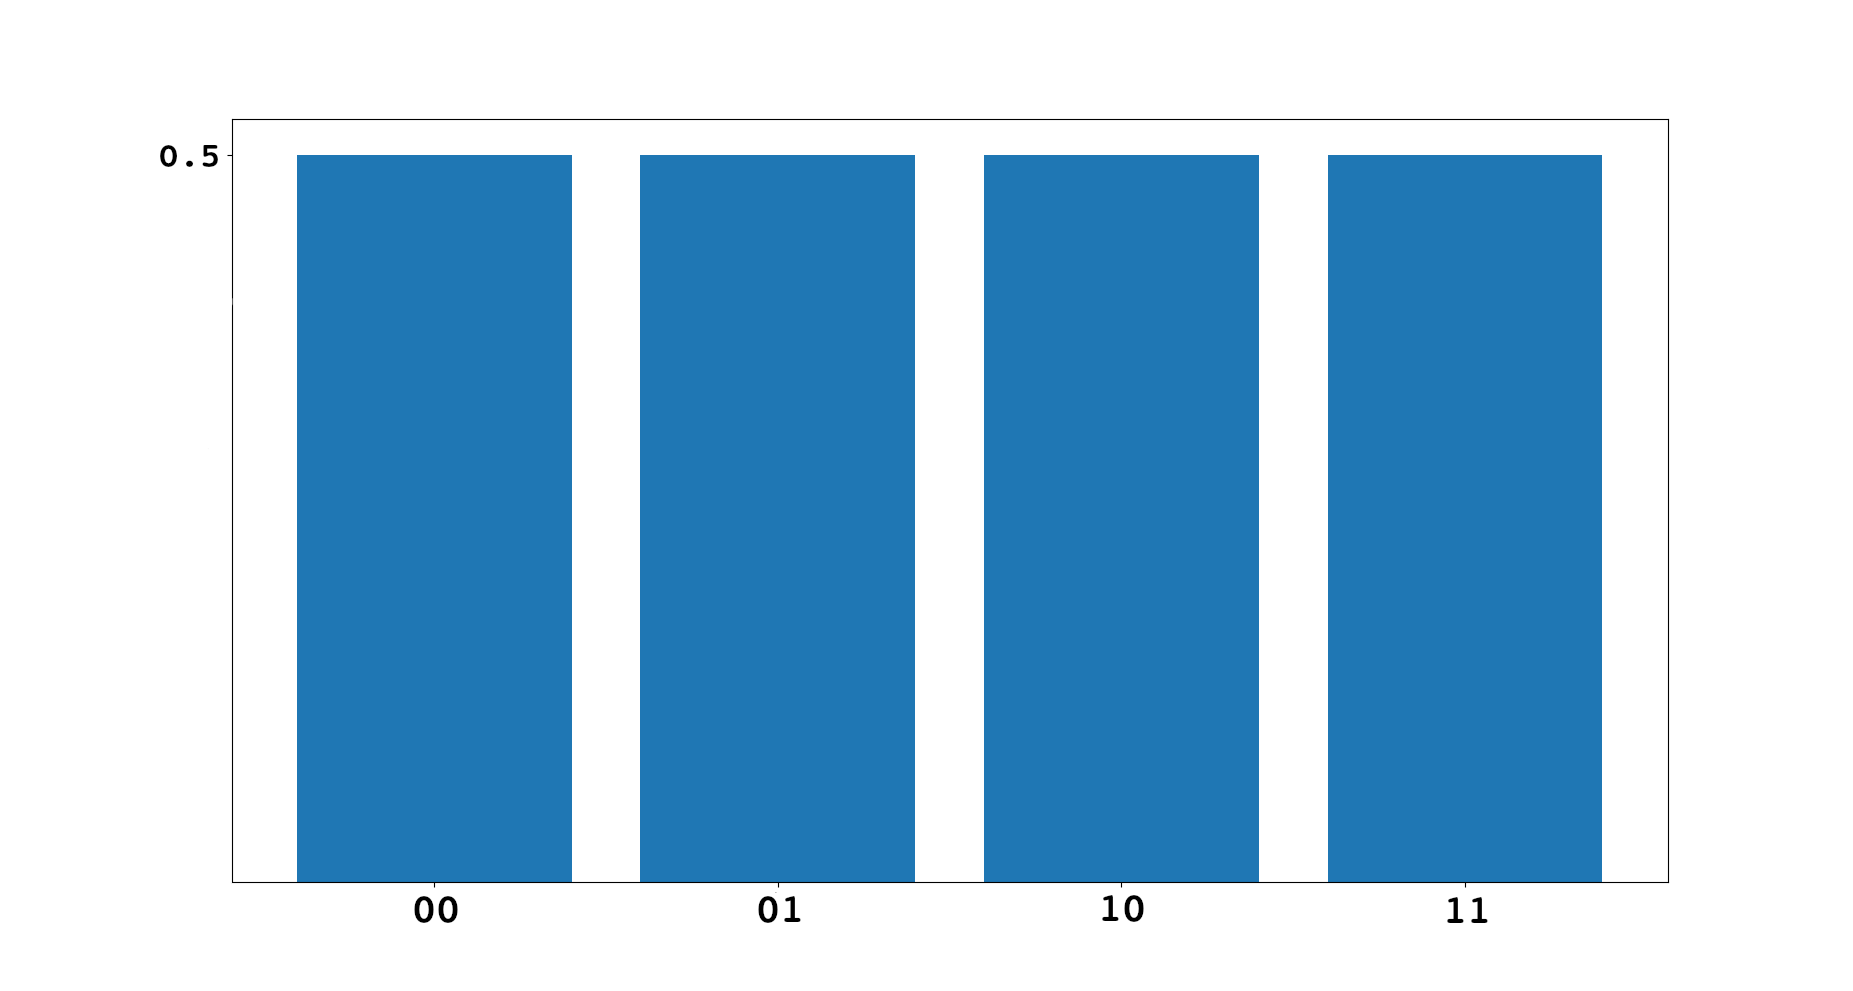
\includegraphics[scale=0.25]{grover_bars_1}
\caption{The uniform superposition presented on a bar diagram.}
\end{figure}

Let's denote the factors standing next to the states as $c_i$ (where \textit{i} is the index of a state or number, which is stored in it).

Before going further, we need to introduce another assumption. We claim, that we are in possession of a function (given for example by an oracle) which recognizes the number $w$. It will be denoted as

\[ f(x) = \begin{cases}
        0, & if\  x \neq w \\
        1, & if\  x = w
        \end{cases} \]

We are also going to introduce an operator, which uses the above function. It also can be understood as an extension of this function

\[ U_f|x\rangle = \begin{cases}
        |x\rangle, & if\  |x\rangle \neq |w\rangle \\
        -|x\rangle, & if\  |x\rangle = |w\rangle,
        \end{cases} \]

which can be rewritten as 

\[ U_f|x\rangle = (-1)^{f(x)}|x\rangle. \]

Of course we can see, that $U_f|w\rangle = -|w\rangle$.

\begin{remark}
Operator $U_f$ can act differently, than just recognizing a specific number. Another example of it is an operator recognizing numbers divisible by 2.
\end{remark}

Let's say, we are looking for a number 2 in our quantum database. If we apply the $U_f$ operator to our initial state $|\psi_0\rangle$ the factor $c_2$ will become negative, which is shown at the bar diagram below:

\begin{figure}[ht]
\centering
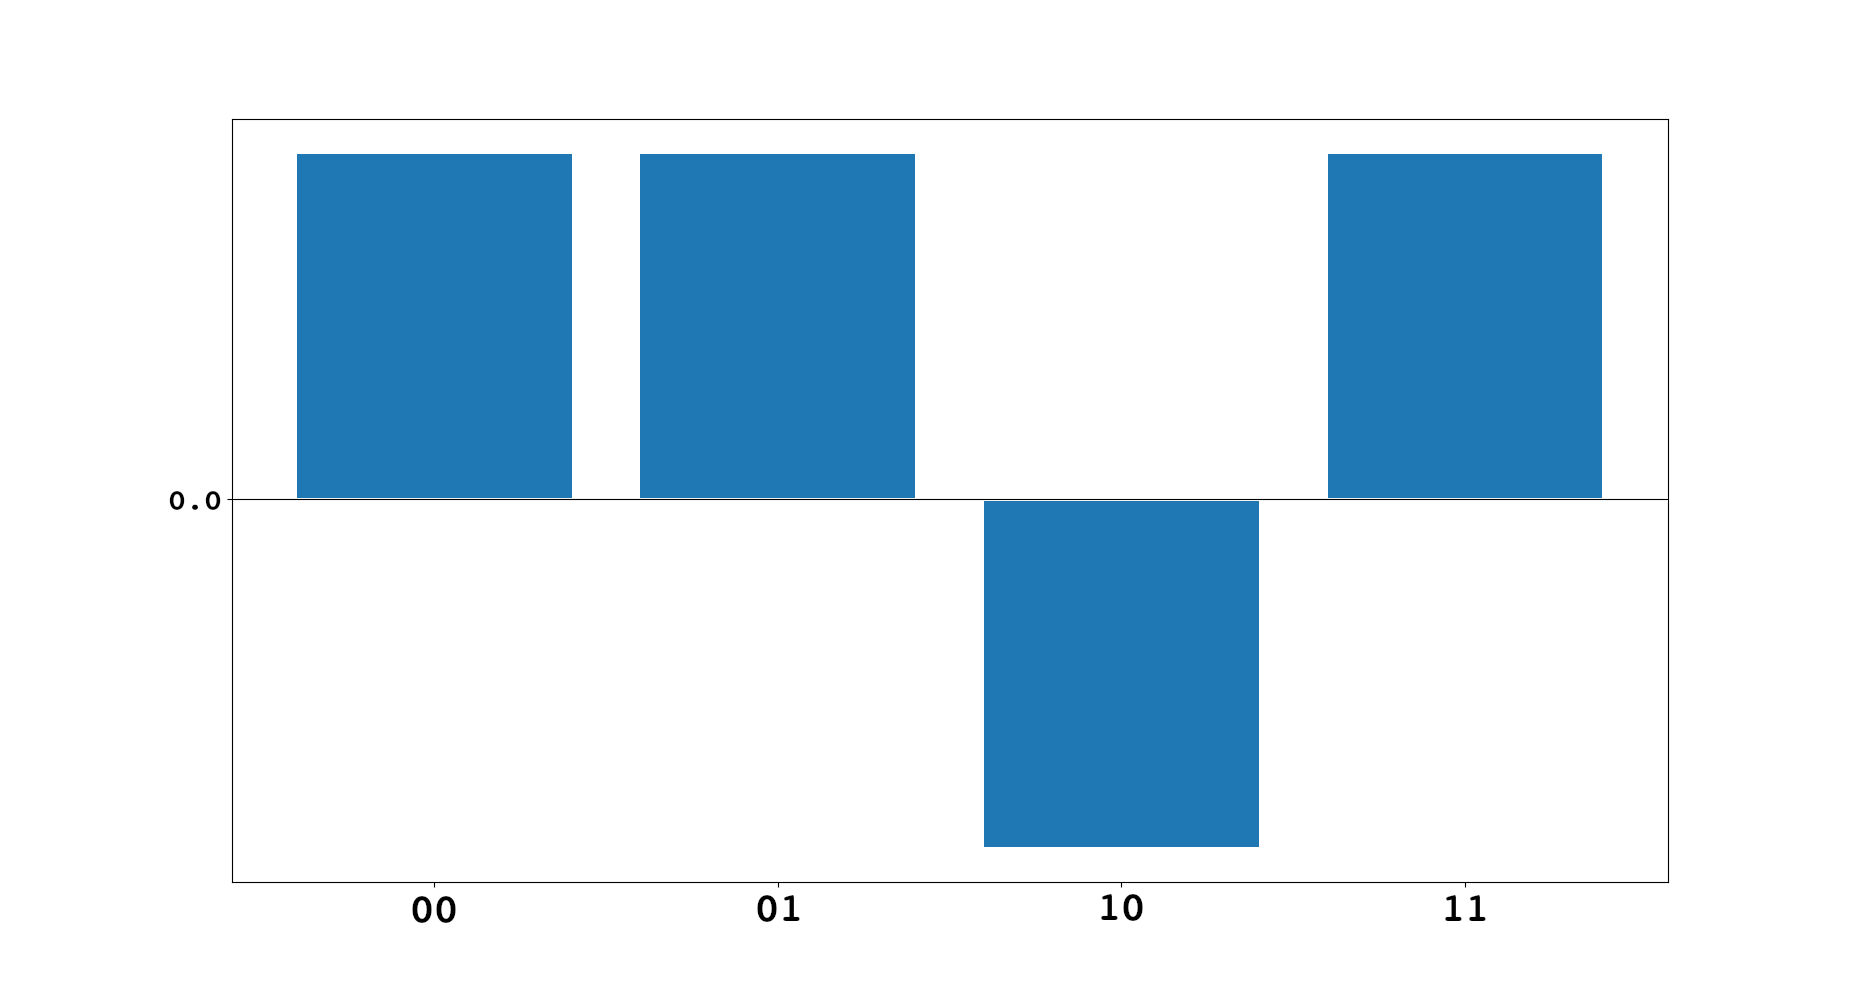
\includegraphics[scale=0.25]{grover_bars_2.png}
\caption{Bar diagram of the vector $U_f|\psi_0\rangle$.}
\end{figure}

\newpage
(this factor can be negative, because during the measurement we will obtain a square of it). The action of the $U_f$ operator can be also understood as a rotation of the vector $|\psi_0\rangle$ along the axis, on which lies the basis vector $|s'\rangle$:

\begin{figure}[ht]
\centering
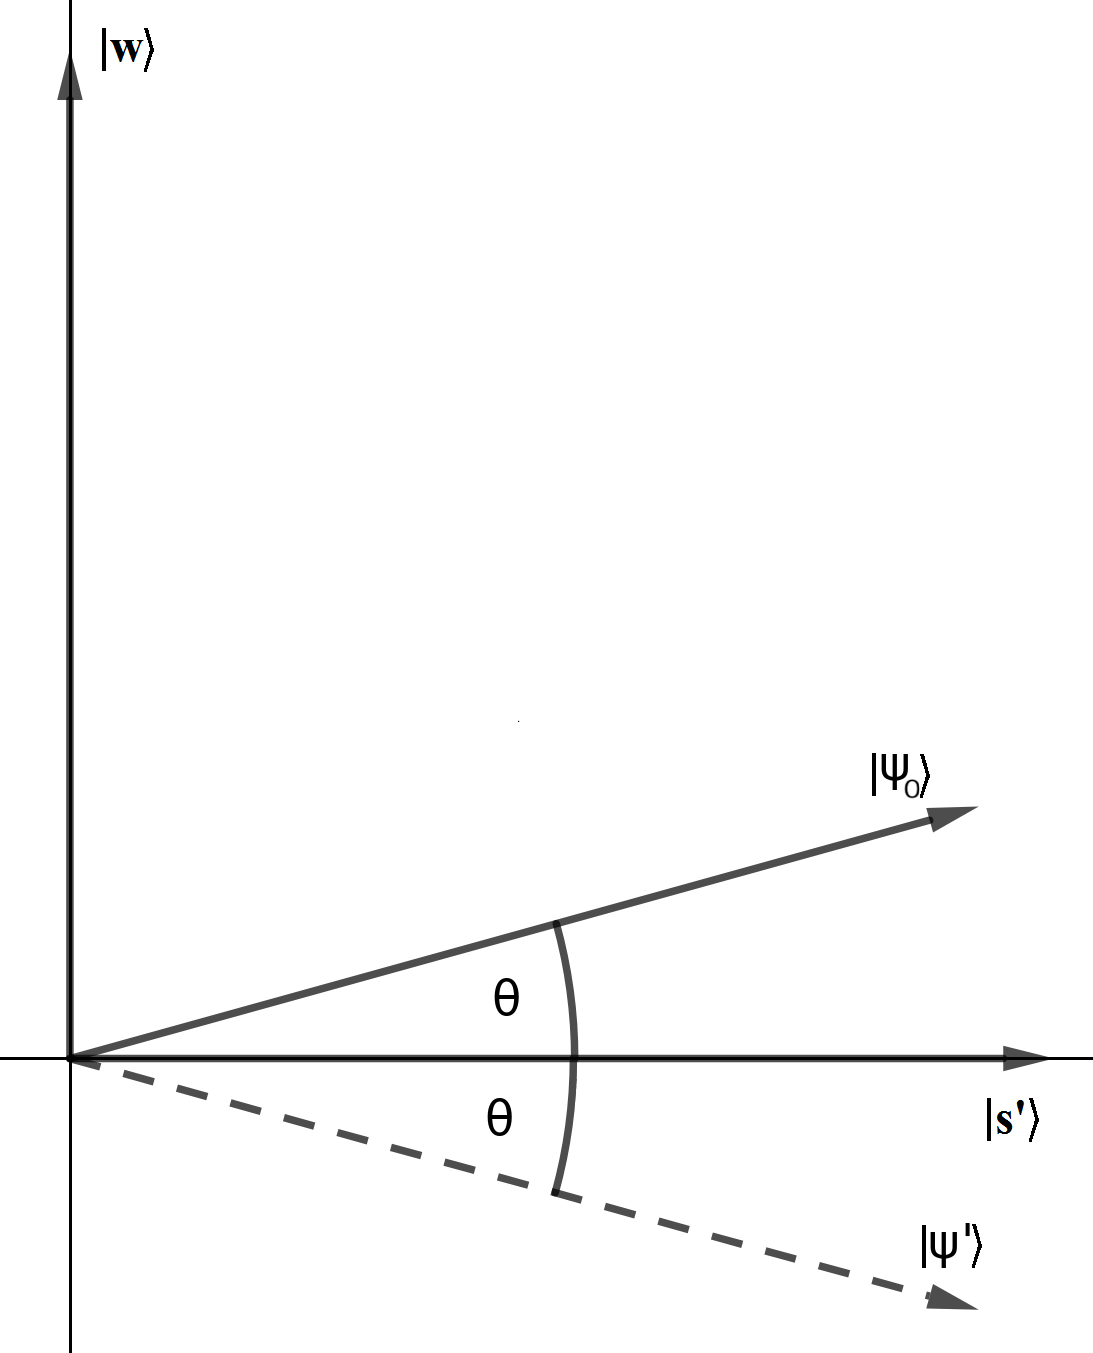
\includegraphics[scale=0.2]{grover_2}
\caption{Action of operator $U_f$ as rotation.}
\end{figure}

The last operator needed in the Grover's algorithm will be denoted as $U_s$. It amplifies factor $c_i$, which are negative and diminishes the positive $c_i$. Action of operator $U_s$ is shown in the bar diagram:

\newpage
\begin{figure}[ht]
\centering
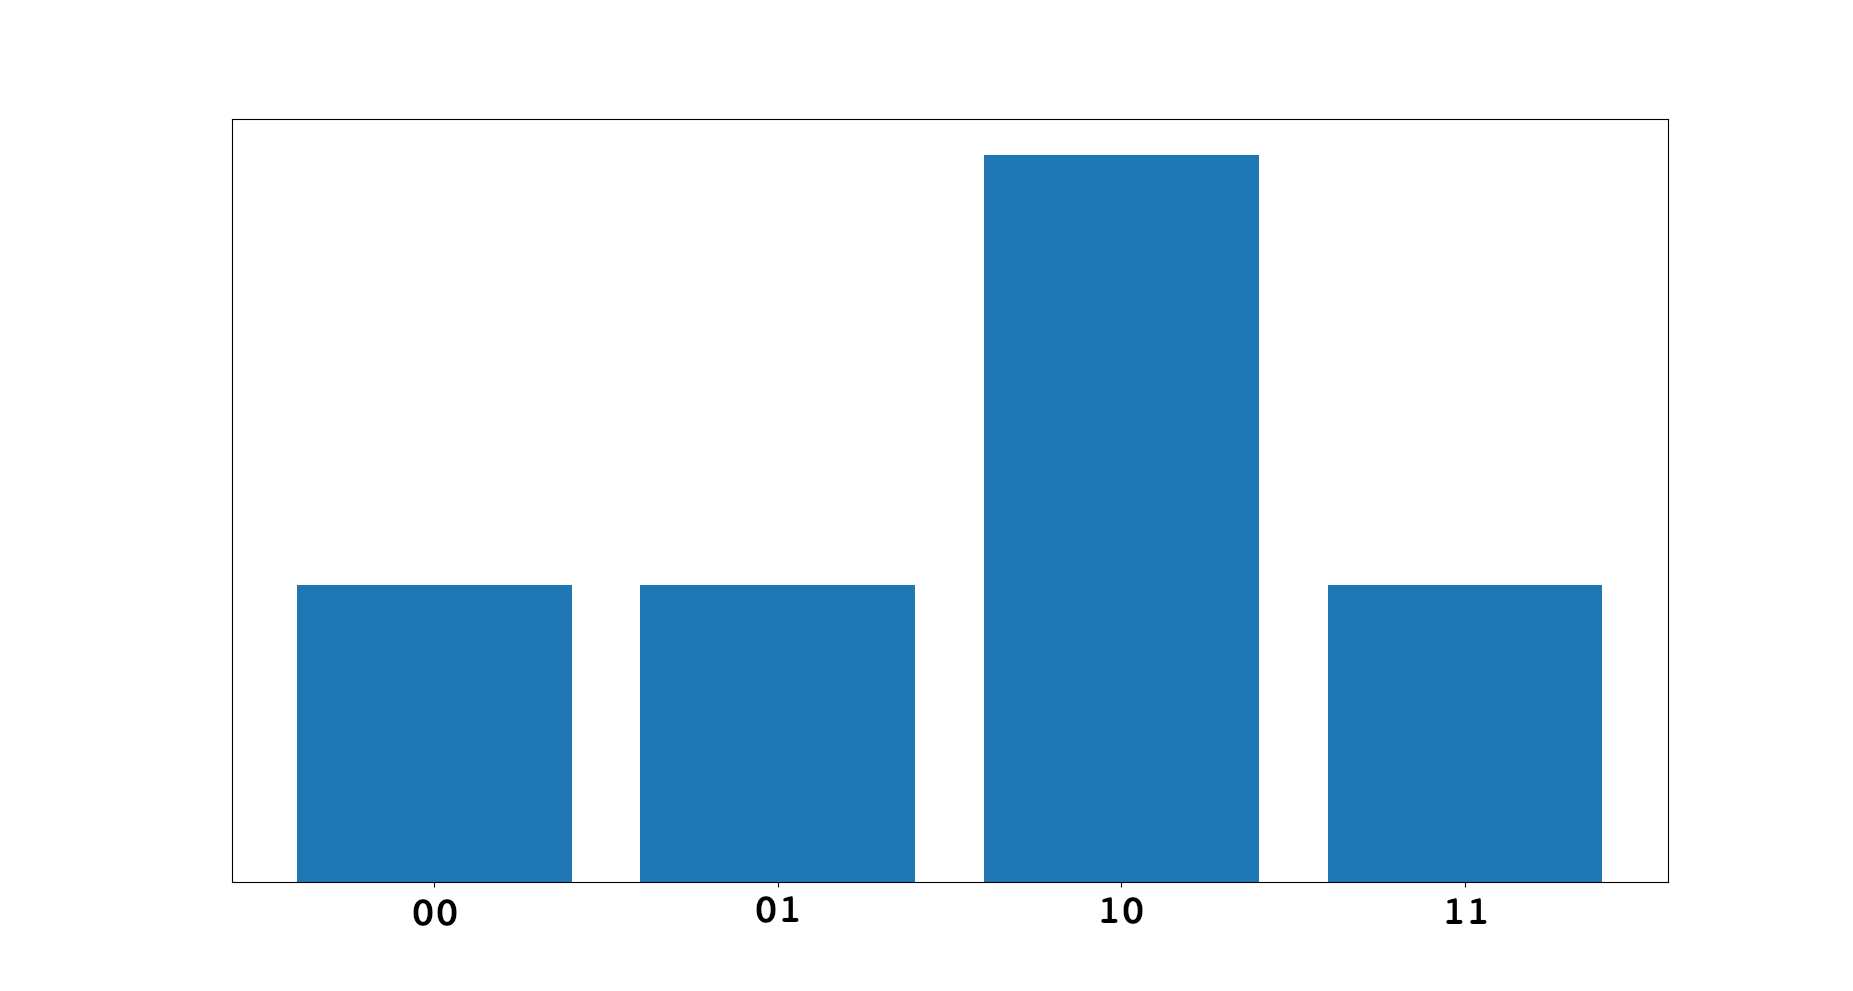
\includegraphics[scale=0.25]{grover_bars_3.png}
\caption{Bar diagram of the vector $U_sU_f|\psi_0\rangle$ (it is not fully correct, which is explained in the below remark).}
\label{grover_bars_3}
\end{figure}

This operator can be also understood as another rotation, but this time it rotates around the average amplitude of all states. It is shown in the picture below:

\begin{figure}[ht]
\centering
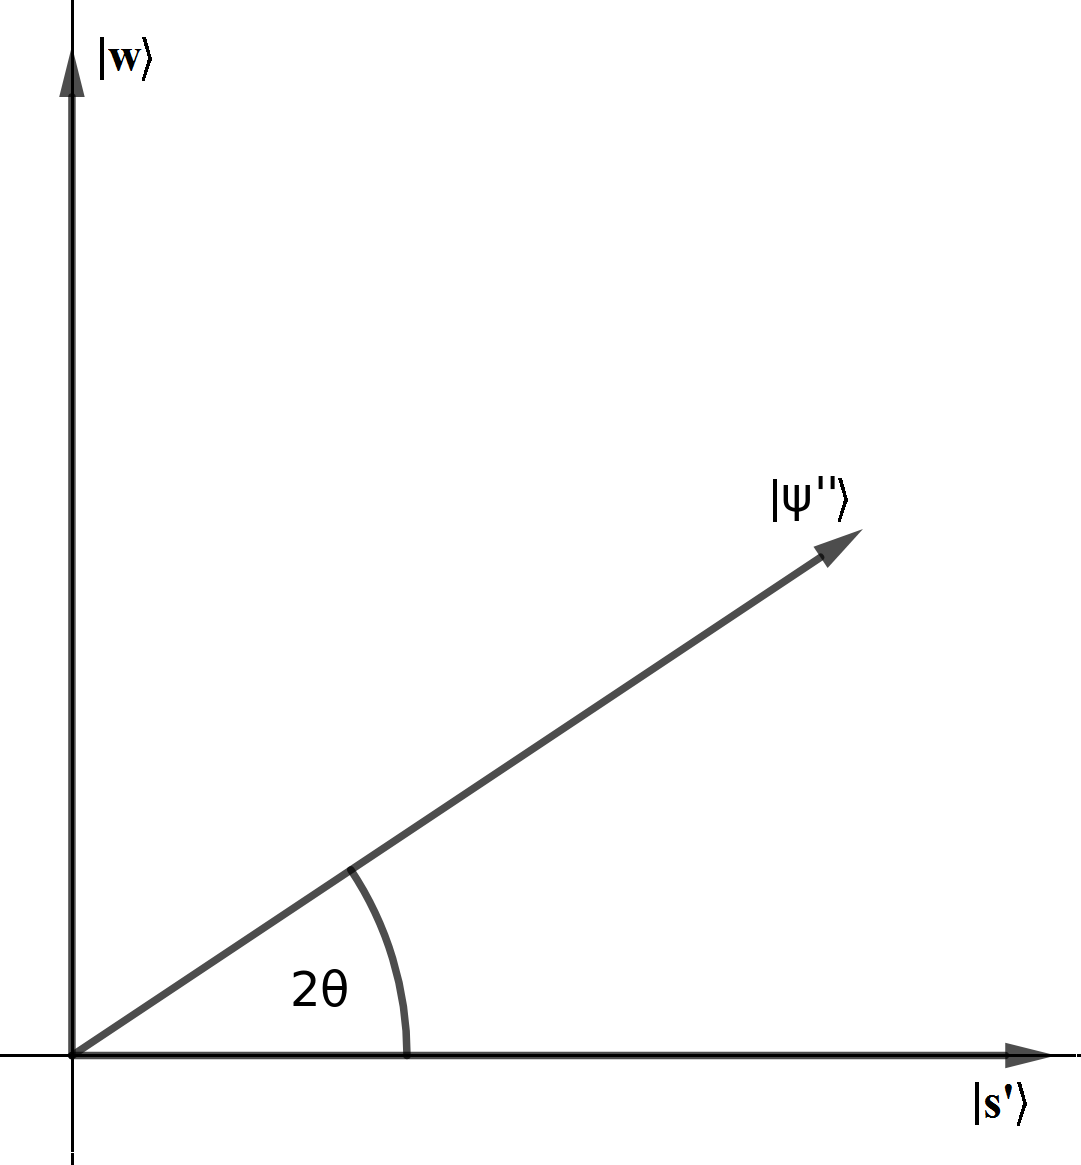
\includegraphics[scale=0.2]{grover_3.png}
\caption{Action of operator $U_s$ as rotation.}
\end{figure}

\begin{remark}
In fact, in our case the average amplitude is equal to $\frac{1}{2}$, so the operator $U_f$ would decrease probabilities $c_0$, $c_1$ and $c_3$ to 0 (because the average amplitude would be exactly in the middle of each of these factors) and increase the $c_2$ to 1 (it cannot be higher, because state vector has to be normalized). The illustration \ref{grover_bars_3} is not fully correct, because factors $c_0$, $c_1$ and $c_2$ should be equal to 0, but it was presented in this way, to give the reader an intuition, of how the $U_s$ operator works.
\end{remark}

Summarizing, Grover's algorithm applies to the initial state operators $U_f$ and $U_s$ as long as the probability of obtaining desired element from database is maximal. In fact, these operations have to applied about $\sqrt{N}$ (where N is the number of elements $N = 2^n$), because using them more than $\sqrt{N}$ times would result in a decrease in probability of obtaining the searched item. This is a great speed-up comparing to the classical algorithms, because the case with uniformly generated calls to a database would result in average cost equal to $\frac{n}{2}$!

The pseudocode of the Grover's algorithm is given below:

\begin{algorithm}[H]
        Initialize the $|\psi_0\rangle$ state (it also can be a result of some other algorithm),\\
        \For{$O(\sqrt{N})$ \  times}{
            \begin{itemize}
                \item apply the $U_f$ operator,
                \item apply the $U_s$ operator,
            \end{itemize}
        }
        measure the resulting state.
 \caption{Pseudocode of the Grover's algorithm}
\end{algorithm}

The implementation of operators $U_f$ and $U_s$ on quantum gates will be presented in the following subsections. At this point we will only point out, that $U_s$ can be obtained by

\[ U_s = 2|s\rangle \langle s| - \mathbb{1},\]

which can be expanded as

\[ U_s = 2 \begin{pmatrix} \frac{1}{\sqrt{N}} \\ \frac{1}{\sqrt{N}} \\ \vdots \\ \frac{1}{\sqrt{N}} \end{pmatrix} \begin{pmatrix} \frac{1}{\sqrt{N}} & \frac{1}{\sqrt{N}} & \hdots & \frac{1}{\sqrt{N}} \end{pmatrix} - \begin{pmatrix} 1 & 0 & \hdots & 0 \\ 0 & 1 & & & \\ \vdots & & \ddots & \\ 0 & & & 1 \end{pmatrix} = \]

\[ 2 \begin{pmatrix} \frac{1}{N} & \frac{1}{N} & \hdots & \frac{1}{N} \\ \frac{1}{N} & \frac{1}{N} & & & \\ \vdots & & \ddots & \\ \frac{1}{N} & & & \frac{1}{N} \end{pmatrix} - \begin{pmatrix} 1 & 0 & \hdots & 0 \\ 0 & 1 & & & \\ \vdots & & \ddots & \\ 0 & & & 1 \end{pmatrix} = \]

\[\begin{pmatrix} \frac{2 - N}{N} & \frac{2}{N} & \hdots & \frac{2}{N} \\ \frac{2}{N} & \frac{2 - N}{N} & & & \\ \vdots & & \ddots & \\ \frac{2}{N} & & & \frac{2 - N}{N} \end{pmatrix}\]

\begin{example}
We will now show the example of searching for a number 2 in our quantum database. We will be using 2 qubits, so we obtain total amount of possible numbers to store equal $N = 2^n = 4$.

Initially, each qubit is in state $|0\rangle$, so the state of the whole system is equal to

\[ |0\rangle \otimes |0\rangle = \begin{pmatrix} 1 \\ 0 \end{pmatrix} \otimes \begin{pmatrix} 1 \\ 0 \end{pmatrix} = \begin{pmatrix} 1 \\ 0 \\ 0 \\ 0 \end{pmatrix}\]

First step is to apply Hadamard gate to each of the qubits. We create $H^{\otimes 2}$ as follows:

\[ H \otimes H = \frac{1}{\sqrt{2}} \begin{pmatrix} 1 & 1 \\ 1 & -1 \end{pmatrix} \otimes \frac{1}{\sqrt{2}} \begin{pmatrix} 1 & 1 \\ 1 & -1 \end{pmatrix} = \frac{1}{2} \begin{pmatrix} 1 & 1 & 1 & 1 \\ 1 & -1 & 1 & -1 \\ 1 & 1 & -1 & -1 \\ 1 & -1 & -1 & 1\end{pmatrix}\]

Now we use the $H^{\otimes 2}$ gate on the $|\psi_0\rangle$ state

\[ |\psi_0\rangle = H^{\otimes 2} |00\rangle = \frac{1}{2} \begin{pmatrix} 1 & 1 & 1 & 1 \\ 1 & -1 & 1 & -1 \\ 1 & 1 & -1 & -1 \\ 1 & -1 & -1 & 1\end{pmatrix} \cdot \begin{pmatrix} 1 \\ 0 \\ 0 \\ 0 \end{pmatrix} = \frac{1}{2} \begin{pmatrix} 1 \\ 1 \\ 1 \\ 1 \end{pmatrix}\]

Each $c_i$ factor is equal to $\frac{1}{2}$, so we obtained the uniform superposition. Now we will use the operator $U_f$. For the purpose of this example we will assume, that we are in possession of a black box performing the action of the $U_f$ operator. It should recognize the state $|10\rangle$, which can be written as

\[ |1\rangle \otimes |0\rangle = \begin{pmatrix} 0 \\ 1 \end{pmatrix} \otimes \begin{pmatrix} 1 \\ 0 \end{pmatrix} = \begin{pmatrix} 0 \\ 0 \\ 1 \\ 0 \end{pmatrix},\]

so it should change the value on the third index in the $|\psi_0\rangle$ vector:

\[ |\psi'\rangle = U_f |\psi_0\rangle = \frac{1}{2}\begin{pmatrix} 1 \\ 1 \\ -1 \\ 1 \end{pmatrix}. \]

We have, that $N = 4$, so the $U_s$ operator is in the form

\[ U_s = \begin{pmatrix} \frac{2 - 4}{4} & \frac{2}{4} & \frac{2}{4} & \frac{2}{4} \\ \\ \frac{2}{4} & \frac{2 - 4}{4} & \frac{2}{4} & \frac{2}{4} \\ \\ \frac{2}{4} & \frac{2}{4} & \frac{2 - 4}{4} & \frac{2}{4} \\ \\ \frac{2}{4} & \frac{2}{4} & \frac{2}{4} & \frac{2 - 4}{4} \end{pmatrix} = \begin{pmatrix} -\frac{1}{2} & \frac{1}{2} & \frac{1}{2} & \frac{1}{2} \\ \\ \frac{1}{2} & -\frac{1}{2} & \frac{1}{2} & \frac{1}{2} \\ \\ \frac{1}{2} & \frac{1}{2} & -\frac{1}{2} & \frac{1}{2} \\ \\ \frac{1}{2} & \frac{1}{2} & \frac{1}{2} & -\frac{1}{2} \end{pmatrix}\]

We apply the $U_s$ operator to the $|\psi'\rangle$ state:

\[ |\psi''\rangle = \begin{pmatrix} -\frac{1}{2} & \frac{1}{2} & \frac{1}{2} & \frac{1}{2} \\ \\ \frac{1}{2} & -\frac{1}{2} & \frac{1}{2} & \frac{1}{2} \\ \\ \frac{1}{2} & \frac{1}{2} & -\frac{1}{2} & \frac{1}{2} \\ \\ \frac{1}{2} & \frac{1}{2} & \frac{1}{2} & -\frac{1}{2} \end{pmatrix} \cdot \frac{1}{2}\begin{pmatrix} 1 \\ 1 \\ -1 \\ 1 \end{pmatrix} =  \frac{1}{4} \begin{pmatrix} -1 & 1 & 1 & 1 \\ 1 & -1 & 1 & 1 \\ 1 & 1 & -1 & 1 \\ 1 & 1 & 1 & -1 \end{pmatrix} \cdot \begin{pmatrix} 1 \\ 1 \\ -1 \\ 1 \end{pmatrix} = \begin{pmatrix} 0 \\ 0 \\ 1 \\ 0 \end{pmatrix}\]

After applying measurement we would obtain state $|10\rangle$ with probability equal to 1. In our example just one iteration was enough to obtain the best possible result.

But let's see what happens, if we apply the whole procedure one more time. We are using $U_f$ on the $|\psi''\rangle$ state and obtain

\[ |\psi'''\rangle = U_f |\psi''\rangle = \begin{pmatrix} 0 \\ 0 \\ -1 \\ 0 \end{pmatrix}. \]

Then, we are using the $U_s$ operator on the $|\psi'''\rangle$ state and get

\[ U_s|\psi'''\rangle = \frac{1}{2}\begin{pmatrix} -1 & 1 & 1 & 1 \\ 1 & -1 & 1 & 1 \\ 1 & 1 & -1 & 1 \\ 1 & 1 & 1 & -1 \end{pmatrix} \cdot \begin{pmatrix} 0 \\ 0 \\ -1 \\ 0 \end{pmatrix} = \begin{pmatrix} -\frac{1}{2} \\ \\ -\frac{1}{2} \\ \\ \frac{1}{2} \\ \\ -\frac{1}{2}  \end{pmatrix}, \]

so the probability, that the system will collapse in any of the possible states is equal to $\frac{1}{4}$. This shows, that using the whole procedure too many times decreases the probability of getting desired element from a quantum database.
\end{example}

\subsection{Implementation of the $U_f$ operator}

In this subsection we will show how to implement on quantum gates a simple operator recognizing a specific number (although, as mentioned before, it is possible to create a function with a wider application). In fact, such an operator can be made out of $C^nZ$ gate with additional \textit{X} gates surrounding the control qubits, which are supposed to be in the $|0\rangle$ state (when considering a register with $n + 1$ qubits).

Based on the above statement we present the quantum circuit recognizing the $|101\rangle$ number:

\[  \scalebox{1.5}{\Qcircuit @C=1em @R=1em {
 & \qw & \ctrl{2} & \qw & \qw \\
 & \gate{X} & \ctrl{1} & \gate{X} & \qw \\
 & \qw & \gate{Z} & \qw & \qw
}} \]

It might be difficult to physically implement the $C^n Z$ gate, so we can decompose this circuit using a borrowed qubit, basing on the knowledge from the second chapter:

\begin{table}[ht]
\centering
\begin{tikzpicture}
\node (a) at (-40,0){
\scalebox{1.3}{\Qcircuit @C=1em @R=1em {
 & \qw & \ctrl{2} & \qw & \qw \\
 & \gate{X} & \ctrl{1} & \gate{X} & \qw \\
 & \qw & \gate{Z} & \qw & \qw
}}
};
\node[yshift=-3.5cm] (b) at (a.south) 
{
\scalebox{1.3}{\Qcircuit @C=1em @R=1em {
 & \lstick{|BO_1\rangle} & \qw & \targ & \ctrl{3} & \targ & \qw & \qw \\
 & & \qw & \ctrl{-1} & \qw & \ctrl{-1} & \qw & \qw \\
 & & \gate{X} & \ctrl{-2} & \qw & \ctrl{-2} & \gate{X} & \qw \\
 & & \qw & \qw & \gate{Z} & \qw & \qw & \qw \\
}}
};
\draw[->,ultra thick](a)--(b);
\end{tikzpicture}
\label{my-label}
\end{table}

Let's try to write this quantum circuit as a matrix. Firstly, we will add the identity gates where it is necessary:

\begin{table}[ht]
\centering
\begin{tikzpicture}
\node (a) at (-40,0){
\scalebox{1.3}{\Qcircuit @C=1em @R=1em {
 & \qw & \ctrl{2} & \qw & \qw \\
 & \gate{X} & \ctrl{1} & \gate{X} & \qw \\
 & \qw & \gate{Z} & \qw & \qw
}}
};
\node[xshift=3.5cm] (b) at (a.east) 
{
\scalebox{1.3}{\Qcircuit @C=1em @R=1em {
 & \gate{I} & \ctrl{2} & \gate{I} & \qw \\
 & \gate{X} & \ctrl{1} & \gate{X} & \qw \\
 & \gate{I} & \gate{Z} & \gate{I} & \qw
}}
};
\draw[->,ultra thick](a)--(b);
\end{tikzpicture}
\label{my-label}
\end{table}

The first layer can be written as

\[ C_1 = I \otimes X \otimes I = \begin{pmatrix} 1 & 0 \\ 0 & 1 \end{pmatrix} \otimes \begin{pmatrix} 0 & 1 \\ 1 & 0 \end{pmatrix} \otimes \begin{pmatrix} 1 & 0 \\ 0 & 1 \end{pmatrix} = \]

\[ \begin{pmatrix} 0 & 1 & 0 & 0 \\ 1 & 0 & 0 & 0 \\ 0 & 0 & 0 & 1 \\ 0 & 0 & 1 & 0 \end{pmatrix} \otimes \begin{pmatrix} 1 & 0 \\ 0 & 1 \end{pmatrix} = \]

\[ \begin{pmatrix}
0 & 0 & 1 & 0 & 0 & 0 & 0 & 0 \\
0 & 0 & 0 & 1 & 0 & 0 & 0 & 0 \\
1 & 0 & 0 & 0 & 0 & 0 & 0 & 0 \\
0 & 1 & 0 & 0 & 0 & 0 & 0 & 0 \\
0 & 0 & 0 & 0 & 0 & 0 & 1 & 0 \\
0 & 0 & 0 & 0 & 0 & 0 & 0 & 1 \\
0 & 0 & 0 & 0 & 1 & 0 & 0 & 0 \\
0 & 0 & 0 & 0 & 0 & 1 & 0 & 0
\end{pmatrix}\]

The second layer consists only of the $C^2Z$ gate, which can be written as

\[ \begin{pmatrix}
1 & 0 & 0 & 0 & 0 & 0 & 0 & 0 \\
0 & 1 & 0 & 0 & 0 & 0 & 0 & 0 \\
0 & 0 & 1 & 0 & 0 & 0 & 0 & 0 \\
0 & 0 & 0 & 1 & 0 & 0 & 0 & 0 \\
0 & 0 & 0 & 0 & 1 & 0 & 0 & 0 \\
0 & 0 & 0 & 0 & 0 & 1 & 0 & 0 \\
0 & 0 & 0 & 0 & 0 & 0 & 1 & 0 \\
0 & 0 & 0 & 0 & 0 & 0 & 0 & -1
\end{pmatrix} \]

The last layer is the same as the first one, so we already have a matrix for it. Now lets multiply all of these matrices to obtain our desired $U_f$ matrix

\[ U_f = C_1 \cdot C^2Z \cdot C_1 = \]

\[ \begin{pmatrix}
0 & 0 & 1 & 0 & 0 & 0 & 0 & 0 \\
0 & 0 & 0 & 1 & 0 & 0 & 0 & 0 \\
1 & 0 & 0 & 0 & 0 & 0 & 0 & 0 \\
0 & 1 & 0 & 0 & 0 & 0 & 0 & 0 \\
0 & 0 & 0 & 0 & 0 & 0 & 1 & 0 \\
0 & 0 & 0 & 0 & 0 & 0 & 0 & 1 \\
0 & 0 & 0 & 0 & 1 & 0 & 0 & 0 \\
0 & 0 & 0 & 0 & 0 & 1 & 0 & 0
\end{pmatrix} \cdot \begin{pmatrix}
1 & 0 & 0 & 0 & 0 & 0 & 0 & 0 \\
0 & 1 & 0 & 0 & 0 & 0 & 0 & 0 \\
0 & 0 & 1 & 0 & 0 & 0 & 0 & 0 \\
0 & 0 & 0 & 1 & 0 & 0 & 0 & 0 \\
0 & 0 & 0 & 0 & 1 & 0 & 0 & 0 \\
0 & 0 & 0 & 0 & 0 & 1 & 0 & 0 \\
0 & 0 & 0 & 0 & 0 & 0 & 1 & 0 \\
0 & 0 & 0 & 0 & 0 & 0 & 0 & -1
\end{pmatrix} \cdot \begin{pmatrix}
0 & 0 & 1 & 0 & 0 & 0 & 0 & 0 \\
0 & 0 & 0 & 1 & 0 & 0 & 0 & 0 \\
1 & 0 & 0 & 0 & 0 & 0 & 0 & 0 \\
0 & 1 & 0 & 0 & 0 & 0 & 0 & 0 \\
0 & 0 & 0 & 0 & 0 & 0 & 1 & 0 \\
0 & 0 & 0 & 0 & 0 & 0 & 0 & 1 \\
0 & 0 & 0 & 0 & 1 & 0 & 0 & 0 \\
0 & 0 & 0 & 0 & 0 & 1 & 0 & 0
\end{pmatrix} = \]

\[
\begin{pmatrix}
1 & 0 & 0 & 0 & 0 & 0 & 0 & 0 \\
0 & 1 & 0 & 0 & 0 & 0 & 0 & 0 \\
0 & 0 & 1 & 0 & 0 & 0 & 0 & 0 \\
0 & 0 & 0 & 1 & 0 & 0 & 0 & 0 \\
0 & 0 & 0 & 0 & 1 & 0 & 0 & 0 \\
0 & 0 & 0 & 0 & 0 & -1 & 0 & 0 \\
0 & 0 & 0 & 0 & 0 & 0 & 1 & 0 \\
0 & 0 & 0 & 0 & 0 & 0 & 0 & 1
\end{pmatrix}
\]

Let's check, if this matrix works as we want it to. It should recognize the $|101\rangle$ state, which can be written as

\[ |101\rangle = \begin{pmatrix} 0 \\ 1 \end{pmatrix} \otimes \begin{pmatrix} 1 \\ 0 \end{pmatrix} \otimes \begin{pmatrix} 0 \\ 1 \end{pmatrix} = \begin{pmatrix} 0 \\ 0 \\ 0 \\ 0 \\ 0 \\ 1 \\ 0 \\ 0 \end{pmatrix}\]

We can see, that our matrix in fact flips the amplitude of probability of such a vector

\[ U_f |101\rangle = \begin{pmatrix}
1 & 0 & 0 & 0 & 0 & 0 & 0 & 0 \\
0 & 1 & 0 & 0 & 0 & 0 & 0 & 0 \\
0 & 0 & 1 & 0 & 0 & 0 & 0 & 0 \\
0 & 0 & 0 & 1 & 0 & 0 & 0 & 0 \\
0 & 0 & 0 & 0 & 1 & 0 & 0 & 0 \\
0 & 0 & 0 & 0 & 0 & -1 & 0 & 0 \\
0 & 0 & 0 & 0 & 0 & 0 & 1 & 0 \\
0 & 0 & 0 & 0 & 0 & 0 & 0 & 1
\end{pmatrix} \cdot \begin{pmatrix} 0 \\ 0 \\ 0 \\ 0 \\ 0 \\ 1 \\ 0 \\ 0 \end{pmatrix} = \begin{pmatrix} 0 \\ 0 \\ 0 \\ 0 \\ 0 \\ -1 \\ 0 \\ 0 \end{pmatrix},\]

which proves, that the whole structure is correct.

\begin{remark}
If, for some reason, we were unable to use the \textit{Z} gate, it could be replaced by \textit{HXH} gates:

\[ HXH = \frac{1}{\sqrt{2}} \begin{pmatrix} 1 & 1 \\ 1 & -1 \end{pmatrix} \cdot \frac{1}{\sqrt{2}}\begin{pmatrix} 0 & 1 \\ 1 & 0 \end{pmatrix} \cdot \begin{pmatrix} 1 & 1 \\ 1 & -1 \end{pmatrix} = \begin{pmatrix} 1 & 0 \\ 0 & -1 \end{pmatrix} = Z.\]

The same works in the other way - we can replace the \textit{X} gate with \textit{HZH} gates:

\[ HZH = \frac{1}{\sqrt{2}} \begin{pmatrix} 1 & 1 \\ 1 & -1 \end{pmatrix} \cdot \begin{pmatrix} 1 & 0 \\ 0 & -1 \end{pmatrix} \cdot \frac{1}{\sqrt{2}} \begin{pmatrix} 1 & 1 \\ 1 & -1 \end{pmatrix} = \begin{pmatrix} 0 & 1 \\ 1 & 0 \end{pmatrix} = X.\]

\end{remark}

\subsection{Implementation of the $-U_s$ operator}

In this subsection we will show how to implement the $-U_s$ operator. Its action will be the same as the $U_s$ operator, with the only difference being a "\textit{-}" sign next to probability amplitudes, which does not change the results of measurement, because we are always obtaining state with the probability equal to square of the amplitude.

The $-U_s$ operator can be created in the following way:

\[ -U_s = H^{\otimes n} X^{\otimes n} C^{n-1}Z X^{\otimes n} H^{\otimes n}.\]

An example quantum circuit with three qubits is given below

\[ \scalebox{1.5}{\Qcircuit @C=1em @R=.7em {
& \multigate{2}{H^{\otimes 3}} & \multigate{2}{X^{\otimes 3}} & \ctrl{2} & \multigate{2}{X^{\otimes 3}} & \multigate{2}{H^{\otimes 3}} & \qw \\
& \ghost{H^{\otimes 3}} & \ghost{X^{\otimes 3}} & \ctrl{1} & \ghost{X^{\otimes 3}} & \ghost{H^{\otimes 3}} & \qw \\
& \ghost{H^{\otimes 3}} & \ghost{X^{\otimes 3}} & \gate{Z} & \ghost{X^{\otimes 3}} & \ghost{H^{\otimes 3}} & \qw
}} \]

It can be decomposed using one borrowed qubit:

\[ \scalebox{1.5}{\Qcircuit @C=1em @R=.7em {
& \lstick{|BO_1\rangle} & \qw & \qw & \targ & \ctrl{3} & \targ & \qw & \qw & \qw \\
& & \multigate{2}{H^{\otimes 3}} & \multigate{2}{X^{\otimes 3}} & \ctrl{-1} & \qw & \ctrl{-1} & \multigate{2}{X^{\otimes 3}} & \multigate{2}{H^{\otimes 3}} & \qw \\
& & \ghost{H^{\otimes 3}} & \ghost{X^{\otimes 3}} & \ctrl{-2} & \qw & \ctrl{-2} & \ghost{X^{\otimes 3}} & \ghost{H^{\otimes 3}} & \qw \\
& & \ghost{H^{\otimes 3}} & \ghost{X^{\otimes 3}} & \qw & \gate{Z} & \qw & \ghost{X^{\otimes 3}} & \ghost{H^{\otimes 3}} & \qw
}} \]

Let's write all layers of this circuit in the matrix form:

\[ H^{\otimes 3} = \frac{1}{2\sqrt{2}}\begin{pmatrix}
1 & 1 & 1 & 1 & 1 & 1 & 1 & 1 \\
1 & -1 & 1 & -1 & 1 & -1 & 1 & -1 \\
1 & 1 & -1 & -1 & 1 & 1 & -1 & -1 \\
1 & -1 & -1 & 1 & 1 & -1 & -1 & 1 \\
1 & 1 & 1 & 1 & -1 & -1 & -1 & -1 \\
1 & -1 & 1 & -1 & -1 & 1 & -1 & 1 \\
1 & 1 & -1 & -1 & -1 & -1 & 1 & 1 \\
1 & -1 & -1 & 1 & -1 & 1 & 1 & -1 
\end{pmatrix}\]

\[ X^{\otimes 3} = \begin{pmatrix}
0 & 0 & 0 & 0 & 0 & 0 & 0 & 1 \\
0 & 0 & 0 & 0 & 0 & 0 & 1 & 0 \\
0 & 0 & 0 & 0 & 0 & 1 & 0 & 0 \\
0 & 0 & 0 & 0 & 1 & 0 & 0 & 0 \\
0 & 0 & 0 & 1 & 0 & 0 & 0 & 0 \\
0 & 0 & 1 & 0 & 0 & 0 & 0 & 0 \\
0 & 1 & 0 & 0 & 0 & 0 & 0 & 0 \\
1 & 0 & 0 & 0 & 0 & 0 & 0 & 0
\end{pmatrix}\]

\[ C^2 Z = \begin{pmatrix}
1 & 0 & 0 & 0 & 0 & 0 & 0 & 0 \\
0 & 1 & 0 & 0 & 0 & 0 & 0 & 0 \\
0 & 0 & 1 & 0 & 0 & 0 & 0 & 0 \\
0 & 0 & 0 & 1 & 0 & 0 & 0 & 0 \\
0 & 0 & 0 & 0 & 1 & 0 & 0 & 0 \\
0 & 0 & 0 & 0 & 0 & 1 & 0 & 0 \\
0 & 0 & 0 & 0 & 0 & 0 & 1 & 0 \\
0 & 0 & 0 & 0 & 0 & 0 & 0 & -1
\end{pmatrix} \]

All of these combined give us the final matrix

\[ -U_s = H^{\otimes n} X^{\otimes n} C^{n-1}Z X^{\otimes n} H^{\otimes n} = \frac{1}{4}\begin{pmatrix}
3 & -1 & -1 & -1 & -1 & -1 & -1 & -1 \\
-1 & 3 & -1 & -1 & -1 & -1 & -1 & -1 \\
-1 & -1 & 3 & -1 & -1 & -1 & -1 & -1 \\
-1 & -1 & -1 & 3 & -1 & -1 & -1 & -1 \\
-1 & -1 & -1 & -1 & 3 & -1 & -1 & -1 \\
-1 & -1 & -1 & -1 & -1 & 3 & -1 & -1 \\
-1 & -1 & -1 & -1 & -1 & -1 & 3 & -1 \\
-1 & -1 & -1 & -1 & -1 & -1 & -1 & 3 \\
\end{pmatrix} \]

Let's see this matrix in action. By applying $H^{\otimes 3}$ gate to the initial $|000\rangle$ state we are getting the uniform superposition:

\[ H^{\otimes 3} |000\rangle = \frac{1}{2\sqrt{2}}\begin{pmatrix}
1 \\ 1 \\ 1 \\ 1 \\ 1 \\ 1 \\ 1 \\ 1
\end{pmatrix}.\]

After applying the $U_f$ operator we are obtaining the state

\[ \frac{1}{2\sqrt{2}}\begin{pmatrix}
1 \\ 1 \\ 1 \\ 1 \\ 1 \\ -1 \\ 1 \\ 1
\end{pmatrix}.\]

Finally, using the $-U_s$ matrix gives us

\[ -U_s \frac{1}{2\sqrt{2}}\begin{pmatrix} 1 \\ 1 \\ 1 \\ 1 \\ 1 \\ -1 \\ 1 \\ 1 \end{pmatrix} = \frac{1}{4\sqrt{2}}\begin{pmatrix}
-1 \\ -1 \\ -1 \\ -1 \\ -1 \\ -5 \\ -1 \\ -1 \end{pmatrix}.\]

If we apply the $U_f$ and $-U_s$ operators one more time we will obtain the best possible outcome for the case with three qubits:

\[ -U_s U_f \frac{1}{4\sqrt{2}}\begin{pmatrix} -1 \\ -1 \\ -1 \\ -1 \\ -1 \\ -5 \\ -1 \\ -1 \end{pmatrix} = 
\frac{1}{8\sqrt{2}} \begin{pmatrix}
-1 \\ -1 \\ -1 \\ -1 \\ -1 \\ 11 \\ -1 \\ -1 \end{pmatrix}\]

\subsection{Final version of the Grover's algorithm}

We have shown all steps needed to construct the Grover's algorithm. Its pseudocode is written below

\begin{algorithm}[H]
    Apply the $H^{\otimes n}$ gate to the initial $|00...0\rangle$ state to obtain uniform superposition, \\
    generate a binary representation of searched number, \\
    \For{$O(\sqrt{N})$ \  times}{
        \begin{itemize}
            \item add the $C^{n-1}Z$ gate and surround control qubits, which are supposed to be equal to 0, with \textit{X} gates,
            \item add the $H^{\otimes n}$ gate,
            \item add the $X^{\otimes n}$ gate,
            \item add the $C^{n-1}Z$ gate,
            \item add the $X^{\otimes n}$ gate,
            \item add the $H^{\otimes n}$ gate,
        \end{itemize}
    }
    measure the resulting state.
 \caption{Pseudocode of the Grover's algorithm for a uniform superposition}
\end{algorithm}

Full code of the program using \textit{qiskit} is presented in the appendix \ref{appendixA}. An example quantum circuit, compatible with the above pseudocode, is given below (for $n = 3$, $U_f$ finding the number 0 and only one iteration of the algorithm):

\[  \scalebox{1.5}{\Qcircuit @C=1em @R=1em {
    & \gate{H} & \gate{X} & \ctrl{2} & \gate{X} & \gate{H} & \gate{X} & \ctrl{2} & \gate{X} & \gate{H} & \qw \\
    & \gate{H} & \gate{X} & \ctrl{1} & \gate{X} & \gate{H} & \gate{X} & \ctrl{1} & \gate{X} & \gate{H} & \qw \\
    & \gate{H} & \gate{X} & \gate{Z} & \gate{X} & \gate{H} & \gate{X} & \gate{Z} & \gate{X} & \gate{H} & \qw \gategroup{1}{3}{3}{5}{.7em}{--} \gategroup{1}{6}{3}{10}{.7em}{--}
}} \]

Groups of gates (surrounded with dashed lines) create the $U_f$ and $-U_s$ operators accordingly. As mentioned earlier, it might be hard to physically implement the $C^n Z$ gate, but we can use one borrowed qubit to modify the above circuit:

\[  \scalebox{1.5}{\Qcircuit @C=1em @R=1em {
    & \qw & \qw & \targ & \ctrl{3} & \targ & \qw & \qw & \qw & \targ & \ctrl{3} & \targ & \qw & \qw & \qw \\
    & \gate{H} & \gate{X} & \ctrl{-1} & \qw & \ctrl{-1} & \gate{X} & \gate{H} & \gate{X} & \ctrl{-1} & \qw & \ctrl{-1} & \gate{X} & \gate{H} & \qw \\
    & \gate{H} & \gate{X} & \ctrl{-2} & \qw & \ctrl{-2} & \gate{X} & \gate{H} & \gate{X} & \ctrl{-2} & \qw & \ctrl{-2} & \gate{X} & \gate{H} & \qw \\
    & \gate{H} & \gate{X} & \qw & \gate{Z} & \qw & \gate{X} & \gate{H} & \gate{X} & \qw & \gate{Z} & \qw & \gate{X} & \gate{H} & \qw \gategroup{1}{3}{4}{7}{.7em}{--} \gategroup{1}{8}{4}{14}{.7em}{--}
}} \]

\[\]

According to the \ref{grover_general}, the above version of Grover's algorithm would work for any initial state (not an uniform superposition), being e.g. result of some other algorithm. Moreover, it is possible to implement quantum algorithm finding minimum in a quantum database (\ref{grover_minimum}). These properties can give a massive speedup in finding solutions of \textit{NP} problems. Let's say, we are trying to find solution to a traveling salesman problem. We could insert lengths of all of the possible routes in a quantum database and use Grover's algorithm, to find the minimum. This leads us to conclusion, that Grover's algorithm can find solutions to \textit{NP} problems in $O(\sqrt{n}$ time (assuming, that we can efficiently create initial quantum state)!

Experimental results for Grover's algorithm are given in the appendix \ref{appendixB}.

\newpage
\section{Algorithms based on the quantum Fourier transform}

We will begin this section by introducing the quantum Fourier transform. We will tell about differences, when comparing it to the classical Fourier transform and show, how it can be implemented on quantum gates. Further, we will gradually present three algorithms basing on this structure: phase estimation, order finding and Shor's factoring algorithms. given these algorithms as a template we will tell about a whole class of algorithms based on quantum Fourier transform. Finally, we will show in detail how Shor's factoring algorithm can be implemented on a quantum computer and present some experimental results.

\subsection{Quantum Fourier transform}

Classical Fourier transform can be understood as a change of basis (its rotation), in which a vector is represented. In this work we will only consider a discrete case of this operation. Mentioned vector can be written as a sequence of complex numbers ${x_i} = (x_1, x_2, ..., x_N)$. \textbf{Discrete Fourier transform} (denoted also as \textbf{DFT}) changes each of vector's components into the new sequence ${y_i} = (y_1, y_2, ..., y_N)$ according to the below formula:

\[ y_k = \frac{1}{\sqrt{N}}\sum_{j = 0}^{N - 1} x_j \cdot e^{-\frac{2 \pi i}{N}jk} = \frac{1}{\sqrt{N}}\sum_{j = 0}^{N - 1} x_j \cdot \bigg[cos\bigg(\frac{2 \pi jk}{N} \bigg) - i \cdot sin\bigg(\frac{2 \pi jk}{N}\bigg)\bigg],\]

where the last transition is based on Euler's formula.

\begin{remark}
Vectors $b_k = (\frac{1}{\sqrt{N}} e^{\frac{2 \pi i}{N} jk} | j = 0, 1, ..., N - 1)^T$ form an orthonormal basis:

\[ \langle b_k | b_{k'} \rangle = \sum_{j = 0}^{N - 1} \bigg(\frac{1}{\sqrt{N}} e^{\frac{2 \pi i}{N}jk}\bigg) \cdot \bigg(\frac{1}{\sqrt{N}} e^{-\frac{2 \pi i}{N}jk'}\bigg) =  \frac{1}{N} \sum_{j = 0}^{N - 1} e^{\frac{2 \pi i}{N} (k - k')j}\]

Now we will consider two cases of the above equation. First case, when $k = k'$ gives us the following result
\[ \frac{1}{N} \sum_{j = 0}^{N - 1} e^{\frac{2 \pi i}{N} 0 \cdot j} = \frac{1}{N} \sum_{j = 0}^{N - 1} 1 = \frac{1}{N} \cdot N = 1. \]

In the other case, when $k \neq k'$ lets denote the result of subtraction $k - k'$ by \textit{t} (so \textit{t} is an integer). Using the formula for the sum of a geometric series we obtain 

\[\frac{1}{N} \sum_{j = 0}^{N - 1} e^{\frac{2 \pi i}{N} t j} = \frac{1 - e^{\frac{2t \pi i}{N}\cdot N}}{1 - e^{\frac{2t \pi i}{N}}} = \frac{1 - e^{2t \pi i}}{1 - e^{\frac{2t \pi i}{N}}}.\]

From the Euler's formula we know, that $e^{2\pi i} = 1$:

\begin{figure}[ht]
\centering
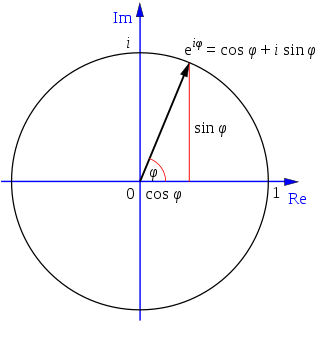
\includegraphics[scale=0.4]{eulers_formula}
\caption{Interpretation of the Euler's formula.}
\end{figure}

\newpage
An integer \textit{t} in the exponent does not change the final result (it can be understood as making many circles around the axes intersection instead of just one). This gives us, that

\[\frac{1 - e^{2t \pi i}}{1 - e^{\frac{2t \pi i}{N}}} = \frac{1 - 1}{1 - e^{\frac{2t \pi i}{N}}} = 0.\]

When we combine the above two cases we see, that the equation from which we started can be written as

\[ \langle b_k | b_{k'} \rangle = \frac{1}{N} \sum_{j = 0}^{N - 1} e^{\frac{2 \pi i}{N} (k - k')j} = \frac{1}{N} \cdot N \cdot \delta_{kk'} = \delta_{kk'}, \]

which proves, that basis vectors $\{b_k\}$ create an orthonormal basis. At the same time we have shown, that discrete Fourier transform (with the $\frac{1}{\sqrt{N}}$ factor) is an \textbf{unitary operation}. Without the $\frac{1}{\sqrt{N}}$ factor this operation would not be unitary.
\end{remark}

The \textbf{quantum Fourier transform} (denoted also as \textbf{QFT}) is an extension of the discrete Fourier transform. It takes into account only vectors of length $N = 2^n$, where \textit{n} is the number of qubits, which we will be using. Qubits create workspace for this operation and, as we stated in the first chapter, when we are considering a compound physical system made of smaller ones, we are using tensor product to describe its behavior. This let's us deduce, that adding a new qubit to the workspace doubles its size. At the same time we are not losing the possibility to transform vectors with odd number of components. We can fill the "missing spaces" with zeroes and use the QFT.

QFT is changing the basis $\{|j\rangle \} = \{ |0\rangle, |1\rangle, ..., |N - 1\rangle \}$ into the new one, similarly to the DFT:

\[ |j\rangle \xrightarrow{\text{QFT}} \frac{1}{\sqrt{N}} \sum_{k = 0}^{N - 1} e^{\frac{2 \pi i}{N} jk} |k\rangle.\]

Other way to write the action of the QFT is given below:

\[ \sum_{j = 0}^{N - 1}x_j |j\rangle \xrightarrow{\text{QFT}} \sum_{k = 0}^{N - 1} y_k |k\rangle,\]

where

\[ y_k = \frac{1}{\sqrt{N}} \sum_{j = 0}^{N - 1} e^{\frac{2 \pi i}{N}jk} x_j.\]

\subsection{Product representation of the quantum Fourier transform}

Before going to the implementation, let's introduce some notation and facts, which will be necessary in this process:

\begin{enumerate}
    \item $N = 2^n$, so the basis consists of states $|0\rangle, |1\rangle, ..., |2^n - 1\rangle$,
    \item binary representation of a number \textit{j} will be denoted as $j = j_1 j_2 ... j_n$, which means
    \[ j = j_1 2^{n - 1} + j_2 2^{n - 2} + ... + j_{n - 1} 2 ^1 + j_n 2^0,\]
    \item notation $0.j_l j_{l+1} ... j_m$ represents $\frac{j_l}{2^1} + \frac{j_{l+1}}{2^2} + ... + \frac{j_{m - 1}}{2^{m - l}} + \frac{j_m}{2^{m - l + 1}}$.
\end{enumerate}

Now we will derive to the result of the QFT acting on given state. This resulting representation will allow us to create a proper quantum circuit. According to the definition, the QFT acting on state $|j\rangle$ can be written as

\[ QFT\ |j\rangle = QFT\ |j_1j_2...j_n\rangle = \frac{1}{2^{\frac{n}{2}}} \sum_{k = 0}^{2^n - 1} e^{\frac{2 \pi ijk}{2^n}} |k\rangle = \]
\[ \frac{1}{2^{\frac{n}{2}}} \sum_{k = 0}^{2^n - 1} e^{\frac{2 \pi ij}{2^n} \sum_{l = 1}^{n}k_l 2^{n - l}} |k_1 k_2 ... k_n\rangle = \]
\[ \frac{1}{2^{\frac{n}{2}}} \sum_{k = 0}^{2^n - 1} e^{2 \pi ij \sum_{l = 1}^{n}k_l 2^{-l}} |k_1 k_2 ... k_n\rangle. \]

Above we replaced $|j\rangle$ and $|k\rangle$ with their binary representations $|j_1j_2...j_n\rangle$ and $|k_1k_2...k_n\rangle$ respectively.

Now we will try to replace the sum $\sum_{k = 0}^{2^n - 1}$ with some other construct. It is important to notice, that in this sum we are going over all of the numbers $0, 1, 2, ..., 2^n - 1$. These numbers can be written in binary form using always \textit{n} bits. Therefore, going through all of these numbers is equivalent to using all of the possible combinations of \textit{n} bits, which can be written as $\sum_{k_1 = 0}^{1}\sum_{k_2 = 0}^{1} ... \sum_{k_n = 0}^{1}$. Finally

\[ \sum_{k = 0}^{2^n - 1} = \sum_{k_1 = 0}^{1} \sum_{k_2 = 0}^{1} ... \sum_{k_n = 0}^{1}.\]

We will use this fact to further decompose considered equation:

\[ \frac{1}{2^{\frac{n}{2}}} \sum_{k = 0}^{2^n - 1} e^{2 \pi ij \sum_{l = 1}^{n}k_l 2^{-l}} |k_1 k_2 ... k_n\rangle = \]
\[ \frac{1}{2^{\frac{n}{2}}} \sum_{k_1 = 0}^{1}\sum_{k_2 = 0}^{1} ... \sum_{k_n = 0}^{1} e^{2 \pi ij \sum_{l = 1}^{n}k_l 2^{-l}} |k_1 k_2 ... k_n\rangle = \]
\[ \frac{1}{2^{\frac{n}{2}}} \sum_{k_1 = 0}^{1}\sum_{k_2 = 0}^{1} ... \sum_{k_n = 0}^{1} e^{2 \pi ij k_1 2^{-1}} \cdot e^{2 \pi ij k_2 2^{-2}} \cdot ... \cdot e^{2 \pi ij k_n 2^{-n}} |k_1 k_2 ... k_n\rangle = \]
\[ \frac{1}{2^{\frac{n}{2}}} \sum_{k_1 = 0}^{1}\sum_{k_2 = 0}^{1} ... \sum_{k_n = 0}^{1} \bigotimes_{l = 1}^{n} e^{2 \pi ij k_l 2^{-l}}|k_l\rangle = \]
\[ \frac{1}{2^{\frac{n}{2}}} \bigotimes_{l=1}^{n} \bigg[ \sum_{k_l = 0}^{1} e^{2 \pi ij k_l 2^{-l}}|k_l\rangle \bigg] = \]
\[ \frac{1}{2^{\frac{n}{2}}} \bigotimes_{l=1}^{n} \bigg[ |0\rangle + e^{2 \pi ij 2^{-l}}|1\rangle \bigg] = \]
\[ \frac{1}{2^{\frac{n}{2}}} \bigotimes_{l=1}^{n} \bigg[ |0\rangle + e^{2 \pi i 2^{-l} \sum_{k = 1}^{n}j_k 2^{n - k}}|1\rangle \bigg] \]

In the last step we just replaced \textit{j} in the exponent by its binary representation. Let's look closer at this exponent. There is a factor $2^{-l}\sum_{k = 1}^{n} j_k 2^{n - k}$, which can be rewritten as

\[ 2^{-l}\sum_{k = 1}^{n} j_k 2^{n - k} = 2^{-l} \bigg( j_1 2^{n - 1} + j_2 2^{n - 2} + ... + j_n 2^0 \bigg) = j_n 2^{-l} + j_{n-1} 2^{-l + 1} + ... + j_1 2^{-l + n - 1}.\]

We also used the tensor product $\bigotimes$ with index \textit{l} going through numbers 1, 2, ..., n. \textit{l} will be at most equal to \textit{n}, so the number $j_n 2^{-l} + j_{n-1} 2^{-l + 1} + ... + j_1 2^{-l + n - 1}$ can be broken down into its integer and fractional parts. For example, for $l = 1$ we obtain

\[ j_{n} 2^{-1} + j_{n-1} 2^{0} + ... + j_{1} 2^{n-2} = 0.j_n + j - 2^{n - 1}, \]

and for $l = 2$ we get

\[ j_{n} 2^{-2} + j_{n-1} 2^{-1} + j_{n-2} 2^{0} + ... + j_{1} 2^{n-3} = 0.j_{n-1} j_n + j - 2^{n - 1} - 2^{n - 2}, \]

where \textit{j} is initial number and $j_i$ are its binary components. Using induction, we can write the final correlation

\[ 2^{-l}\sum_{k = 1}^{n} j_k 2^{n - k} = 0.j_l j_{l+1} ... j_n + \bigg(j - \sum_{i = 0}^{l} j_i 2^{n - 1 - i} \bigg).\]

It is extremely important to notice, for the purpose of further deduction, that part $\bigg(j - \sum_{i = 0}^{l} j_i 2^{n - 1 - i} \bigg)$ \textbf{is an integer}. Because of this we will replace it with symbol \textit{t}, so the upper equation can be rewritten in the form:

\[ 2^{-l}\sum_{k = 1}^{n} j_k 2^{n - k} = 0.j_l j_{l+1} ... j_n + t.\]

Now, let's come back to the whole exponential function, from which we started the above deduction. Having the last statement, we can write, that

\[ e^{2 \pi ij 2^{-l}} = e^{2 \pi i 2^{-l} \sum_{k=1}^{n} j_n 2^{n - k}} = \]
\[ e^{2 \pi i [0.j_l...j_n + (j - \sum_{i = 0}^{l}j_i 2^{n - 1 - i})]} = \]
\[ e^{2 \pi i [0.j_l...j_n + t]} = e^{2 \pi i 0.j_l...j_n} \cdot e^{2 \pi i t}. \]

We have stated, that \textit{t} is an integer. From the Euler's formula we know, that $e^{2 \pi i} = 1$, so number $e^{2 \pi i t}$ will be also equal to 1 (as before, we can interpret this as making many circles around the intersection of axes). Finally we have

\[ e^{2 \pi i j 2^{-l}} = e ^{2 \pi i 0.j_l ... j_n}.\]

\begin{remark}
In the above process we implicitly used the equivalence of usage of different notation. We will show what we mean by this by giving an example. Let's see, what happens with binary representation of number \textit{j} for consecutive values of \textit{l} (we have to remember, that we can ommit the integer part of a number in this reasoning):
\begin{itemize}
    \item l = 1
    \[ j_1 j_2 ... j_n \rightarrow j_1 j_2 ... j_{n-1}.j_n \rightarrow 0.j_n \equiv 0.j_{l'},\  where\ l' = n,\]
    \item l = 2
    \[ j_1 j_2 ... j_n \rightarrow 0.j_{n-1}j_n \equiv 0.j_{l'}j_n,\  where\ l' = n - 1,\]
    $\vdots$ 
    \item l = n - 1
    \[ j_1 j_2 ... j_n \rightarrow 0.j_2 j_3 ... j_n \equiv 0.j_{l'}...j_n,\  where\ l' = 2,\]
    \item l = n
    \[ j_1 j_2 ... j_n \rightarrow 0.j_1 j_2 ... j_n \equiv 0.j_{l'}... j_n,\  where\ l' = 1,\]
\end{itemize}

so we can see, that while considering the final result, which we want to achieve, indices \textit{l} and \textit{l'} can be thought of as equivalent (we only have to reverse the order).
\end{remark}

Using the last received property we can rewrite the equation from which we started:

\[ \frac{1}{2^{\frac{n}{2}}} \bigotimes_{l=1}^{n} \bigg[ |0\rangle + e^{2 \pi i 2^{-l} \sum_{k = 1}^{n}j_k 2^{n - k}}|1\rangle \bigg] = \]
\[ \frac{1}{2^{\frac{n}{2}}} \bigotimes_{l=1}^{n} \bigg[ |0\rangle + e^{2 \pi i 0.j_l ... j_n}|1\rangle \bigg] = \]
\[ \frac{1}{2^{\frac{n}{2}}} \bigg( |0\rangle + e^{2 \pi i 0.j_n}|1\rangle \bigg) \otimes \bigg( |0\rangle + e^{2 \pi i 0.j_{n - 1} j_n}|1\rangle \bigg) \otimes ... \otimes \bigg( |0\rangle + e^{2 \pi i 0.j_1 j_2 ... j_n}|1\rangle \bigg) = \]
\[ \frac{|0\rangle + e^{2 \pi i 0.j_n}|1\rangle}{\sqrt{2}} \otimes \frac{|0\rangle + e^{2 \pi i 0.j_{n - 1} j_n}|1\rangle}{\sqrt{2}} \otimes ... \otimes \frac{|0\rangle + e^{2 \pi i 0.j_1 j_2 ... j_n}|1\rangle}{\sqrt{2}}\]

This final form let's us say that each component of a quantum state $|j\rangle$, that is $|j_1\rangle$, $|j_2\rangle$, ..., $|j_n\rangle$ is transformed into state $\frac{|0\rangle + e^{2 \pi i 0.j_n}|1\rangle}{\sqrt{2}}$, $\frac{|0\rangle + e^{2 \pi i 0.j_{n - 1} j_n}|1\rangle}{\sqrt{2}}$, ..., $\frac{|0\rangle + e^{2 \pi i 0.j_1 j_2 ... j_n}|1\rangle}{\sqrt{2}}$ accordingly. It can be written in the form called \textbf{product representation}:

\[ |j_1 j_2 ... j_n\rangle \xrightarrow{\text{QFT}} \frac{|0\rangle + e^{2 \pi i 0.j_n}|1\rangle}{\sqrt{2}} \otimes \frac{|0\rangle + e^{2 \pi i 0.j_{n - 1} j_n}|1\rangle}{\sqrt{2}} \otimes ... \otimes \frac{|0\rangle + e^{2 \pi i 0.j_1 j_2 ... j_n}|1\rangle}{\sqrt{2}} \]

\subsection{Implementation of the quantum Fourier transform on quantum gates}

In the previous subsection we obtained very powerful tool - the product representation of the quantum Fourier transform. We will use it in the process of implementation of QFT.

To achieve our goal we will use two gates - Hadamard and $R_k$. Just to remind, $R_k$ gate can be written as 

\[ R_k = \begin{pmatrix} 1 & 0 \\ 0 & e^{\frac{2 \pi i}{2^k}}\end{pmatrix}\]

and Hadamard gate as

\[ H = \frac{1}{\sqrt{2}}\begin{pmatrix}
1 & 1 \\ 1 & -1
\end{pmatrix}\]

Action of the Hadamard gate can be also written as

\[ H|0\rangle = \frac{1}{\sqrt{2}}(|0\rangle + |1\rangle) \]
\[ H|1\rangle = \frac{1}{\sqrt{2}}(|0\rangle - |1\rangle) \]

We can write down the action of Hadamard gate acting on the $|j_1\rangle$ state as

\[ H|j_1\rangle = \frac{1}{\sqrt{2}} \bigg( |0\rangle + e^{2 \pi i 0.j_1} |1\rangle \bigg). \]

Let's recall, that components $j_1$ appeared in the binary representation of a number $j$, so only states in which they can be are $|0\rangle$ and $|1\rangle$. For these two states, in which $|j_1\rangle$ can be, we have

\begin{itemize}
    \item $j_1 = 0$
    \[ e^{2 \pi i 0.j_1} = e^{2 \pi i \frac{0}{2}} = e^{0} = 1, \]
    \item $j_1 = 1$
    \[ e^{2 \pi i 0.j_1} = e^{2 \pi i \frac{1}{2}} = e^{\pi i} = -1. \]
\end{itemize}

Now let's look at the circuit below:

\[  \scalebox{1.5}{\Qcircuit @C=1em @R=1em {
 \lstick{|j_2\rangle} & \qw & \ctrl{1} & \qw \\
 \lstick{|j_1\rangle} & \gate{H} & \gate{R_2} & \qw
}} \]

State of the system after going through the first layer of gates is in the state

\[ |\psi_1\rangle = |j_2\rangle \otimes \frac{1}{\sqrt{2}} \bigg( |0\rangle +  e^{2 \pi i 0.j_1} \bigg).\]

Again, $|j_2\rangle$ can be in two states: $|0\rangle$ and $|1\rangle$. Let's investigate action of the second layer in these two cases (remembering, that after going through the first layer qubit $|j_1\rangle$ changes into $|j_1'\rangle = \frac{1}{\sqrt{2}}\bigg( |0\rangle + e^{2 \pi i 0.j_1} \bigg)$):

\begin{itemize}
    \item $|j_2\rangle = |0\rangle$
    \[ |j_2\rangle \otimes |j_1'\rangle = \begin{pmatrix} 0 \\ 1 \end{pmatrix} \otimes \frac{1}{\sqrt{2}}\begin{pmatrix} 1 \\ e^{2 \pi i 0.j_1}\end{pmatrix} = \begin{pmatrix}0 \\ 0 \\ 1 \\  e^{2 \pi i 0.j_1} \end{pmatrix} \]
    \[ CR_k |j_2 j_1'\rangle = \begin{pmatrix} 1 & 0 & 0 & 0 \\ 0 & 1 & 0 & 0 \\ 0 & 0 & 1 & 0 \\ 0 & 0 & 0 & e^{\frac{2 \pi i}{2^k}} \end{pmatrix} \frac{1}{\sqrt{2}}\begin{pmatrix} 0 \\ 0 \\ 1 \\ e^{2 \pi i 0.j_1}\end{pmatrix} = \]
    \[ \frac{1}{\sqrt{2}}\begin{pmatrix} 0 \\ 0 \\ 1 \\ e^{2 \pi i 0.j_1}\cdot e^{\frac{2 \pi i}{2^k}} \end{pmatrix} = \begin{pmatrix} 0 \\ 1 \end{pmatrix} \otimes \frac{1}{\sqrt{2}} \begin{pmatrix} 1 \\ e^{2 \pi i 0.j_1}\cdot e^{\frac{2 \pi i}{2^k}} \end{pmatrix}\]
    \item $|j_2\rangle = |1\rangle$
    \[ |j_2\rangle \otimes |j_1'\rangle = \begin{pmatrix} 1 \\ 0 \end{pmatrix} \otimes \frac{1}{\sqrt{2}}\begin{pmatrix} 1 \\ e^{2 \pi i 0.j_1}\end{pmatrix} = \begin{pmatrix} 1 \\  e^{2 \pi i 0.j_1} \\ 0 \\ 0 \end{pmatrix} \]
    \[ CR_k |j_2 j_1'\rangle = \begin{pmatrix} 1 & 0 & 0 & 0 \\ 0 & 1 & 0 & 0 \\ 0 & 0 & 1 & 0 \\ 0 & 0 & 0 & e^{\frac{2 \pi i}{2^k}} \end{pmatrix} \frac{1}{\sqrt{2}}\begin{pmatrix} 1 \\ e^{2 \pi i 0.j_1} \\ 0 \\ 0 \end{pmatrix} = \frac{1}{\sqrt{2}}\begin{pmatrix} 1 \\ e^{2 \pi i 0.j_1} \\ 0 \\ 0 \end{pmatrix} = \begin{pmatrix} 1 \\ 0 \end{pmatrix} \otimes \frac{1}{\sqrt{2}} \begin{pmatrix} 1 \\ e^{2 \pi i 0.j_1} \end{pmatrix}\]
\end{itemize}

The final state of the second qubit can be written as
\[ \frac{|0\rangle + e^{2 \pi i 0.j_1 + \frac{2 \pi i}{2^k}}}{\sqrt{2}} = \frac{|0\rangle + e^{2 \pi i \bigg( 0.j_1 + \frac{1}{2^k}\bigg)} }{\sqrt{2}}, \]

or

\[ \frac{|0\rangle + e^{2 \pi i 0.j_1}}{\sqrt{2}} = \frac{|0\rangle + e^{2 \pi i \bigg( 0.j_1 + \frac{0}{2^k} \bigg)}}{\sqrt{2}}\]

depending on, in which $|j_2\rangle$ state was. So, we can write down the combined version of the above cases:

\[|j_1''\rangle = \frac{|0\rangle + e^{2 \pi i 0.j_1 00...j_2}}{\sqrt{2}}\]

depending on the $k$ in the $R_k$ gate. For $k = 2$ we get

\[|j_1''\rangle = \frac{|0\rangle + e^{2 \pi i 0.j_1 j_2}}{\sqrt{2}}.\]

We can easily see, that the $R_3$ gate with new control qubit $|j_3\rangle$ would add to the exponent of above formula factor $0.j_3$, gate $R_4$ with control qubit $|j_4\rangle$ factor $0.j_4$ and so on. Having this conclusion we can present final quantum circuit computing QFT:

\newpage
\scalebox{0.85}{\Qcircuit @C=1em @R=1.5em {
\lstick{|j_1\rangle} & \gate{H} & \gate{R_2} & \qw & {\cdots} & & \gate{R_{n-1}} & \gate{R_n} & \qw & \qw & \qw & \qw & \qw & \qw & \qw & \qw & \qw & \qw & \qw & \qw & \qw & \rstick{( |0\rangle + e^{2 \pi i 0.j_1 ... j_n} |1\rangle ) / \sqrt{2}} \\
\lstick{|j_2\rangle} & \qw & \ctrl{-1} & \qw & {\cdots} & & \qw & \qw & \gate{H} & \qw & {\cdots} & & \gate{R_{n-2}} & \gate{R_{n-1}} & \qw & {\cdots} & & \qw & \qw & \qw & \qw & \rstick{( |0\rangle + e^{2 \pi i 0.j_2 ... j_n} |1\rangle ) / \sqrt{2}} \\
\vdots & &  &  &  &  &  &  &  &  &  &  &  &  &  &  & \\ 
 & &  &  &  &  &  &  &  &  &  &  &  &  &  &  & \\ 
\lstick{|j_{n - 1}\rangle} & \qw & \qw & \qw & \qw & \qw & \ctrl{-4} & \qw & \qw & \qw & \qw & \qw & \ctrl{-3} & \qw & \qw & {\cdots} & & \gate{H} & \gate{R_2} & \qw & \qw &  \rstick{( |0\rangle + e^{2 \pi i 0.j_{n-1} j_n} |1\rangle ) / \sqrt{2}} \\
\lstick{|j_n\rangle} & \qw & \qw & \qw & \qw & \qw & \qw & \ctrl{-5} & \qw & \qw & \qw & \qw & \qw & \ctrl{-4} & \qw & {\cdots} & & \qw & \ctrl{-1} & \gate{H} & \qw & \rstick{( |0\rangle + e^{2 \pi i 0.j_n} |1\rangle ) / \sqrt{2}} \\
}}

\[ \]

The above circuit implements the following transformation:

\[ |j_1 j_2 ... j_n\rangle \xrightarrow{\text{QFT}} \frac{|0\rangle + e^{2 \pi i 0.j_1 j_2 ... j_n}|1\rangle}{\sqrt{2}} \otimes \frac{|0\rangle + e^{2 \pi i 0.j_2 ... j_n}|1\rangle}{\sqrt{2}} \otimes ... \otimes  \frac{|0\rangle + e^{2 \pi i 0.j_n}|1\rangle}{\sqrt{2}}\]

Adding at the end of the circuit appropriate swap gates gives us desired product representation of QFT:

\[ |j_1 j_2 ... j_n\rangle \xrightarrow{\text{QFT}} \frac{|0\rangle + e^{2 \pi i 0.j_n}|1\rangle}{\sqrt{2}} \otimes \frac{|0\rangle + e^{2 \pi i 0.j_{n - 1} j_n}|1\rangle}{\sqrt{2}} \otimes ... \otimes \frac{|0\rangle + e^{2 \pi i 0.j_1 j_2 ... j_n}|1\rangle}{\sqrt{2}} \]

Received quantum circuit is of size $O(n)$ (for the input size equal to \textit{n}).


\subsection{Phase estimation algorithm} \label{phase_estimation}

Let's assume, that we are given an operator $U$ (e.g. as an oracle), which for an eigenvector $|u\rangle$ has eigenvalue $e^{2 \pi i \phi}$

\[ U|u\rangle \equiv e^{2 \pi i \phi} |u\rangle\]

Target of the \textbf{phase estimation algorithm} is to calculate the $\phi$ factor in the exponent.

In section \ref{bell_states} we were analyzing circuits in the form

\[  \scalebox{1.5}{\Qcircuit @C=1em @R=1em {
 \lstick{|x\rangle} & \gate{H} & \ctrl{1} & \qw \\
 \lstick{|y\rangle} & \qw & \targ & \qw
}} \]

which were generating Bell states. Let's modify this circuit, by replacing the \textit{CNOT} gate with a $CU$ gate and $|x\rangle$ and $|y\rangle$ states with $|0\rangle$ and $|u\rangle$ states accordingly

\[  \scalebox{1.5}{\Qcircuit @C=1em @R=1em {
 \lstick{|0\rangle} & \gate{H} & \ctrl{1} & \qw & \rstick{\big( |0\rangle + e^{2 \pi i \phi}|1\rangle \big)/\sqrt{2}} \\
 \lstick{|u\rangle} & \qw & \gate{U} & \qw & \rstick{|u\rangle}
}} \]

(we are also assuming, that state $|u\rangle$ can be obtained efficiently e.g. from an oracle).

First of all, we have to deduce the structure of the $U$ operator in the matrix form. We introduce the following notation:

\[ U = \begin{pmatrix} u_1 & u_2 \\ u_3 & u_4 \end{pmatrix}, \ |u\rangle = \begin{pmatrix} a \\ b \end{pmatrix}\]

Moreover, we know, that $U|u\rangle \equiv e^{2 \pi i \phi}|u\rangle$, which can be written as

\[ U|u\rangle \equiv \begin{pmatrix} u_1 & u_2 \\ u_3 & u_4 \end{pmatrix} \cdot \begin{pmatrix} a \\ b \end{pmatrix} \equiv e^{2 \pi i \phi} \begin{pmatrix} a \\ b \end{pmatrix}. \]

The above gives us, that $u_2 = u_3 = 0$ and $u_1 = u_4 = e^{2 \pi i \phi}$. Having this in mind, we can write the $CU$ gate as

\[ CU = \begin{pmatrix} 
1 & 0 & 0 & 0 \\
0 & 1 & 0 & 0 \\
0 & 0 & e^{2 \pi i \phi} & 0 \\
0 & 0 & 0 & e^{2 \pi i \phi}
\end{pmatrix}\]

Just to recall, we can write down the first layer of gates as follows:

\[ H \otimes I = \frac{1}{\sqrt{2}} \begin{pmatrix} 1 & 1 \\ 1 & -1 \end{pmatrix} \otimes \begin{pmatrix} 1 & 0 \\ 0 & 1 \end{pmatrix} = \frac{1}{\sqrt{2}} \begin{pmatrix}
1 & 0 & 1 & 0 \\
0 & 1 & 0 & 1 \\
1 & 0 & -1 & 0 \\
0 & 1 & 0 & -1 \end{pmatrix}\]

Now, let's look at the states, in which the system consisting of considered two qubits is in, after going through each layer of gates:

\[ |\psi_0\rangle = |0\rangle \otimes |u\rangle = \begin{pmatrix} a \\ b \\ 0 \\ 0 \end{pmatrix} \]

\[ |\psi_1\rangle = H \otimes I|\psi_0\rangle = \frac{1}{\sqrt{2}} \begin{pmatrix} a \\ b \\ a \\ b \end{pmatrix} \]

\[ |\psi_2\rangle = CU|\psi_1\rangle = \begin{pmatrix} 
1 & 0 & 0 & 0 \\
0 & 1 & 0 & 0 \\
0 & 0 & e^{2 \pi i \phi} & 0 \\
0 & 0 & 0 & e^{2 \pi i \phi}
\end{pmatrix} \cdot \frac{1}{\sqrt{2}} \begin{pmatrix} a \\ b \\ a \\ b \end{pmatrix} = \frac{1}{\sqrt{2}} \begin{pmatrix}
a \\ b \\ e^{2 \pi i \phi} a \\ e^{2 \pi i \phi} b \end{pmatrix} = \frac{1}{\sqrt{2}} \begin{pmatrix} 1 \\ e^{2 \pi i \phi}\end{pmatrix} \otimes \begin{pmatrix} a \\ b \end{pmatrix} \]

In short, second qubit remained unchanged and first qubit changed its state from $|0\rangle$ to $\frac{|0\rangle + e^{2 \pi i \phi}|1\rangle}{\sqrt{2}}$. This is very interesting behavior, because we are used to the case, in which the control qubit remains unchanged and we operate on a target qubit. In the above case, the target qubit remained unchanged and the control qubit gained some new information!

Now let's extend our assumption, that we can efficiently implement the $U$ operator by saying, that we can do the same for $U^{2^{0}}$, $U^{2^{1}}$, ..., $U^{2^{t - 1}}$, where \textit{t} depends on the accuracy, with which we would like to obtain the $\phi$ factor and probability of successful termination of our algorithm. Having all of the above facts, we present the following circuit:

\[\]

\scalebox{1.5}{\Qcircuit @C=1em @R=1em {
 \lstick{|0\rangle} & \gate{H} & \qw & \qw & \qw & {\cdots} & & \ctrl{4} & \qw & \rstick{\big( |0\rangle + e^{2 \pi i 2^{t - 1}\phi}|1\rangle \big)/\sqrt{2}} \\
 \vdots\\
 \lstick{|0\rangle} & \gate{H} & \qw & \ctrl{2} & \qw & {\cdots} & & \qw & \qw & \rstick{\big( |0\rangle + e^{2 \pi i 2^{1}\phi}|1\rangle \big)/\sqrt{2}} \\
 \lstick{|0\rangle} & \gate{H} & \ctrl{1} & \qw & \qw & {\cdots} & & \qw & \qw & \rstick{\big( |0\rangle + e^{2 \pi i 2^{0}\phi}|1\rangle \big)/\sqrt{2}} \\
 \lstick{|u\rangle} & {/} \qw & \gate{U^{2^{0}}} & \gate{U^{2^{1}}} & \qw & {\cdots} & & \gate{U^{2^{t - 1}}} & \qw & \rstick{|u\rangle}
}}

\[\]

We can decode $\phi$ using \textit{t} bits as $\phi = 0.\phi_1 \phi_2 ... \phi_t$ (we can accomplish this by e.g. dividing $\phi$ by $2^t$). Using this coding, we can rewrite final state of the first register (consisting of qubits, which were initially in state $|0\rangle$) as

\[ \frac{1}{2^{t/2}} \bigg(|0\rangle + e^{2 \pi i 2^{t - 1}\phi}|1\rangle \bigg) \otimes \bigg(|0\rangle + e^{2 \pi i 2^{t - 2}\phi}|1\rangle \bigg) \otimes ... \otimes \bigg(|0\rangle + e^{2 \pi i 2^{0}\phi}|1\rangle \bigg) = \]
\[ \frac{1}{2^{t/2}} \bigg(|0\rangle + e^{2 \pi i 0.\phi_t}|1\rangle \bigg) \otimes \bigg(|0\rangle + e^{2 \pi i 0.\phi_{t-1}\phi_t}|1\rangle \bigg) \otimes ... \otimes \bigg(|0\rangle + e^{2 \pi i 0.\phi_0...\phi_t}|1\rangle \bigg) \]

We could make the above step, because 

\[ 2^{t-1}\phi = 2^{t-1} 0.\phi_1 \phi_2 ... \phi_{t-1} \phi_t = \phi_1\phi_2...\phi_{t-1}.\phi_t \rightarrow 0.\phi_t \]

We could omit the integer part using the same reasoning as in the derivation of QFT circuit.

The final state of our first register is the same as the result, which would give us applying QFT to the state $|\phi\rangle$. Because of this, we can use the \textbf{inverse quantum Fourier transform} to obtain our desired $\phi$. This leads us to final quantum circuit implementing the phase estimation algorithm:


\[ \scalebox{1.5}{\Qcircuit @C=1em @R=1em {
 \lstick{|0\rangle} & {/} \qw & \gate{H^{\otimes t}} &  {^{^{|j\rangle}}} \qw & \ctrl{1} & \qw & \gate{FT^\dagger} & \meter & \qw \\
 \lstick{|u\rangle} & {/} \qw  & \qw & \qw & \gate{U^j} & \qw & \qw & \qw & \qw & \rstick{|u\rangle}
 }} \]

\subsection{Order finding and continued fractions algorithms}

\begin{definition}
For positive integers \textit{x} and \textit{N} (with no common divisors), such that $x < N$, we define an \textbf{order} \textit{r} of \textit{x}, as the least positive integer, for which $x^r \equiv 1 \ (mod\ N)$.
\end{definition}

In this subsection we will show algorithm, which for a given \textit{x} and \textit{N} finds order \textit{r}. It will be an extension of the phase estimation algorithm. Let's start with an assumption, that we are in possession of an operator \textit{U} (e.g from an oracle), which performs the following rotation

\[ U|y\rangle \equiv |xy\ (mod\ N)\rangle,\]

for $y \in \{0, 1\}^L$, $L = \lceil log N \rceil$. We will now prove, that \textit{U} is unitary. 

\begin{proof}
For non-negative numbers $y_1$ and $y_2$ we have

\[ xy_1 \equiv xy_2\ (mod\ N) \Longleftrightarrow \]
\[ x(y_1 - y_2) \equiv 0\ (mod\ N) \Longleftrightarrow \]
\[ y_1 - y_2 \equiv 0\ (mod\ N) \Longleftrightarrow \]
\[ y_1 \equiv y_2\ (mod\ N) \]

We were able to make the second transition (omit the \textit{x} variable), because we stated in the definition, that \textit{x} and \textit{N} have no common divisors. From the ortonormality of basis we have

\[ \langle y_1\ (mod\ N)| y_2\ (mod\ N)\rangle = \begin{cases}
       1,  & if\ y_1 \equiv y_2\ (mod\ N) \\
       0, & otherwise \\
     \end{cases} = \delta_{12}\]

We can also write, that

\[ \langle y_1\ (mod\ N)| y_2\ (mod\ N)\rangle \equiv \]
\[ \langle xy_1\ (mod\ N)| xy_2\ (mod\ N)\rangle = \delta_{12},\]

which proves, that \textit{U} is unitary.
\end{proof}

Now we will find the eigenvector for the operator \textit{U}. Let's note, that vectors

\[ |x^0\rangle,\ |x^1\rangle,\ |x^2\rangle, ...,\ |x^{r-1}\rangle\]

make an orthonormal basis of \textit{r}-dimensional vector subspace \textit{V} of \textit{N}-dimensional vector space, with basis vectors $|0\rangle$, $|1\rangle$, ..., $|N - 1\rangle$. Because

\[ x^{k + r} \equiv x^k\ (mod\ N)\]

and

\[ U|x^k\ (mod\ N)\rangle \equiv |x^{k + 1}\ (mod\ N)\rangle\]

usage of the operator \textit{U} on \textit{V} does not give a vector from outside the space \textit{V} (when the power of \textit{x} goes beyond the size of the space \textit{V}, thanks to modulo operation it still remains in the desired vector space e.g. $x^0 \equiv x^r\ (mod\ N)$, $x^1 \equiv x^{r+1}\ (mod\ N)$ and so on). Let $|u\rangle$ be the eigenvector of the operator \textit{U} with eigenvalue $e^{2 \pi i \phi}$

\[ U|u\rangle \equiv e^{2 \pi i \phi}|u\rangle\]

At this point $|u\rangle$ and $e^{2 \pi i \phi}$ are unknown. We can write down the $|u\rangle$ vector using basis vectors of the \textit{V} space

\[ |u\rangle = \sum_{k = 0}^{r - 1} c_k |x^k\ (mod\ N)\rangle.\]

We can also write the action of the operator \textit{U} using the above procedure:

\[ U|u\rangle = U\sum_{k = 0}^{r - 1} c_k |x^k\ (mod\ N)\rangle \equiv \sum_{k = 0}^{r - 1} c_k |x^{k+1}\ (mod\ N)\rangle.\]

From the equation for the eigenvalue of the operator \textit{U} and the above equation we get

\[ U|u\rangle \equiv e^{2 \pi i \phi}|u\rangle \equiv \sum_{k = 0}^{r - 1} e^{2 \pi i \phi} c_k |x^k\ (mod\ N)\rangle.\]

Let's write an example for $r = 3$:

\[ \sum_{k = 0}^{r - 1} c_k |x^{k+1}\ (mod\ N)\rangle \equiv c_0|x^{0 + 1}\ (mod\ N)\rangle + c_1|x^{1 + 1}\ (mod\ N)\rangle + c_2|x^{2 + 1}\ (mod\ N)\rangle \equiv \]
\[ c_0|x^{1}\ (mod\ N)\rangle + c_1|x^{2}\ (mod\ N)\rangle + c_2|x^{0}\ (mod\ N)\rangle \]

\[ \sum_{k = 0}^{r - 1} e^{2 \pi i \phi} c_k |x^k\ (mod\ N)\rangle \equiv e^{2 \pi i \phi}c_0|x^0\ (mod\ N)\rangle + e^{2 \pi i \phi}c_1|x^1\ (mod\ N)\rangle + e^{2 \pi i \phi}c_2|x^2\ (mod\ N)\rangle.\]

From the equation for the eigenvalue of the operator \textit{U} we have, that two above sums are equal. Because of this, factors next to the basis vectors have to be equal, for example $c_1 = e^{2 \pi i \phi}c_2$. By continuing this reasoning we can write general form for the factor $c_k$:

\[ c_k = e^{2 \pi i \phi} c_{k + 1}.\]

This gives us

\[ c_{k+1} = e^{- 2 \pi i \phi}c_k,\]

from which we get

\[ c_k = e^{- 2 \pi i \phi k} c_0.\]

We have to remember, that vector $|u\rangle$ has to be normalized. Because of this we have

\[ \sum_{k = 0}^{r - 1}|c_k|^2 = 1 \rightarrow \]

\[ \sum_{k = 0}^{r - 1}|e^{- 2 \pi i \phi k}c_0|^2 = \sum_{k = 0}^{r - 1}e^{- 2 \pi i \phi k}e^{2 \pi i \phi k} c_0^2 = \sum_{k = 0}^{r - 1}e^{0} c_0^2 = \sum_{k = 0}^{r - 1} c_0^2 = rc_0^2 = 1\]

The last equation leads us to

\[ rc_0^2 = 1 \rightarrow c_0 = \pm \frac{1}{\sqrt{r}}.\]

\begin{remark}
In fact, $c_0$ can be also written as $c_0 = \pm \frac{1}{\sqrt{r}}e^{i \phi_0}$, where $\phi_0 \in \mathbb{R}$. Phase $e^{i \phi_0}$ would appear next to every coefficient of the state vector e.g. $|x\rangle = \alpha_0 e^{i \phi_0} |0\rangle + e^{i \phi_0}\alpha_1|1\rangle$. But when we measure some observable, we get the results with probability equal to square of the inner product of probability amplitudes, which gives us

\[ |e^{i \phi_0}\alpha_0|^2 = e^{i \phi_0}e^{-i \phi_0}\alpha_0^2 = \alpha_0^2,\]

so the global phase cannot be measured in any experiment.
\end{remark}

Knowing the value of $c_0$ we can write the final form of the eigenvector $|u\rangle$

\[ c_k = \frac{1}{\sqrt{r}} e^{-2 \pi i \phi k} \rightarrow \]

\[ |u\rangle = \frac{1}{\sqrt{r}} \sum_{k = 0}^{r - 1} e^{-2 \pi i \phi k} |x^k\ (mod\ N)\rangle.\]

Now let's look closer at the dependence between \textit{r} and $\phi$. If we apply \textit{U} to its eigenvector \textit{r} times we get

\[ U^r|u\rangle \equiv e^{2 \pi i \phi r}|u\rangle.\]

Let's also rewrite the rotation performed by the operator \textit{U}

\[ U|u\rangle \equiv U \bigg( \frac{1}{\sqrt{r}} \sum_{k = 0}^{r - 1} e^{-2 \pi i \phi k} |x^k\ (mod\ N)\rangle \bigg) \equiv \frac{1}{\sqrt{r}} \sum_{k = 0}^{r - 1} e^{-2 \pi i \phi k} |x^{k+1}\ (mod\ N)\rangle. \]

If we apply \textit{U} two times to its eigenvector we get

\[ U^2|u\rangle \equiv \frac{1}{\sqrt{r}} \sum_{k = 0}^{r - 1} e^{-2 \pi i \phi k} |x^{k+2}\ (mod\ N)\rangle.\] 

Finally applying \textit{U} \textit{r} times to $|u\rangle$ gives

\[ U^r|u\rangle \equiv \frac{1}{\sqrt{r}} \sum_{k = 0}^{r - 1} e^{-2 \pi i \phi k} |x^{k+r}\ (mod\ N)\rangle \equiv \frac{1}{\sqrt{r}} \sum_{k = 0}^{r - 1} e^{-2 \pi i \phi k} |x^k\ (mod\ N)\rangle \equiv |u\rangle.\]

We previously wrote, that $U^r|u\rangle \equiv e^{2 \pi i \phi r}|u\rangle$. These two facts combined give us

\[ e^{2 \pi i \phi r} = 1.\]

By the Euler's formula we know, that $\phi r$ has to be an integer. Because of this, we can introduce a new number $0 \leq s < r - 1$, $s \in \mathbb{Z}$, such that

\[ \phi = \frac{s}{r}.\]

Using \textit{s} we can introduce new notation for eigenvectors of the \textit{U} operator, which have eigenvalue $e^{2 \pi i \phi} = e^{\frac{2 \pi i s}{r}}$. These eigenvectors will be denoted as

\[ |u_s\rangle = \frac{1}{\sqrt{r}} \sum_{k = 0}^{r - 1} e^{-\frac{2 \pi i s k}{r}} |x^k\ (mod\ N)\rangle.\]

Because $\phi = \frac{s}{r}$ we can use the phase estimation to calculate its approximation $\Tilde{\phi} = \Tilde{\frac{s}{r}}$. Having the approximated value of $\Tilde{\phi}$ we can use a classical \textbf{continued fractions algorithm} \cite{nielsen_chuang}, to retrieve \textit{r} (we have to remember, that phase estimation would give us value $2 \pi i \Tilde{\phi}$, from which we have to extract $\Tilde{\phi}$).

Main idea of this algorithm derives from the below form of writing real numbers

\[ [a_0, ..., a_M] \equiv a_0 + \frac{1}{a_1 + \frac{1}{a_2 + \frac{1}{... + \frac{1}{M}}}}, \]

where $[a_0, ..., a_M]$ is a vector of non-negative integers (the \textit{i}-th number in the vector corresponds to the \textit{i}-th fraction in the expansion). In order to use this algorithm we have to determine a step, in which we will stop the expansion of a real number (it will be denoted as \textit{m}). Usage of \textit{m} allow us to write the real number in a form $[a_0, ..., a_m]$ ($0 \leq m \leq M$). Let's look at the example below, to see this algorithm in action.

\begin{example}
Let's say, that the phase estimation algorithm gave us approximated value of $\phi$ equal to $\Tilde{\phi} = 1.26$. We begin expansion of this number:

\[ 1.26 = 1 + \frac{26}{100} = 1 + \frac{1}{\frac{100}{26}} = 1 + \frac{1}{3.85} = 1 + \frac{1}{3 + \frac{85}{100}} = 1 + \frac{1}{3 + \frac{1}{\frac{100}{85}}} = 1 + \frac{1}{3 + \frac{1}{1.18}} = 1 + \frac{1}{3 + \frac{1}{1 + \frac{1}{\frac{100}{18}}}} = 1 + \frac{1}{3 + \frac{1}{1 + \frac{1}{5.55}}}\]

In the above procedure we were expanding fractions only to the second decimal place. In the final step, we will use even bigger approximation and change 5.55 into 5 (it is necessary for the algorithm to be useful). After this change is done we are wrap this form to obtain fraction of two integers:

\[ 1 + \frac{1}{3 + \frac{1}{1 + \frac{1}{5.55}}} \approx 1 + \frac{1}{3 + \frac{1}{1 + \frac{1}{5}}} = 1 + \frac{1}{3 + \frac{5}{6}} = 1 + \frac{1}{\frac{23}{6}} = 1 + \frac{6}{23} = \frac{29}{23}\]

From the initial $\Tilde{\phi} = 1.26$ we obtained, that it can be written as $\frac{29}{23}$ ($ = \frac{s}{r}$), so the desired value of \textit{r} is equal to 23. Moreover, $\frac{29}{23} = 1.26086957$, which shows that this is a great approximation of $\Tilde{\phi}$. 
\end{example}

The last thing that we have to cope with is creation of the eigenvector $|u_s\rangle$ of the \textit{U} operator. It would seem impossible to create such a state without knowing the value of \textit{r}. In fact we will show, that

\[ \frac{1}{\sqrt{r}}\sum_{s = 0}^{r - 1}|u_s\rangle = |1\rangle,\]

so the superposition of all egienvectors of the \textit{U} operator is equal to the state $|1\rangle$.

\begin{proof}
\[ \frac{1}{\sqrt{r}}\sum_{s = 0}^{r - 1}|u_s\rangle = \frac{1}{\sqrt{r}} \sum_{s = 0}^{r - 1} \frac{1}{\sqrt{r}} \sum_{k = 0}^{r - 1} e^{-\frac{2 \pi i k s}{r}} |x^k\ (mod\ N)\rangle = \frac{1}{r} \sum_{k = 0}^{r - 1} \bigg( \sum_{s = 0}^{r - 1} e^{-\frac{2 \pi i k s}{r}} \bigg) |x^k\ (mod\ N)\rangle = \]

\[\frac{1}{r} \bigg[ \sum_{s = 0}^{r - 1} e^0 |x^0\ (mod\ N)\rangle + \sum_{k = 1}^{r - 1}\sum_{s = 0}^{r - 1} e^{-\frac{2 \pi i k s}{r}} |x^k\ (mod\ N)\rangle \bigg] \]

From the formula for the sum of a geometric series we get

\[\frac{1}{r} \bigg[ \sum_{s = 0}^{r - 1} e^0 |x^0\ (mod\ N)\rangle + \sum_{k = 1}^{r - 1}\sum_{s = 0}^{r - 1} e^{-\frac{2 \pi i k s}{r}} |x^k\ (mod\ N)\rangle \bigg]  = \frac{1}{r} \bigg[ r|1\rangle + \sum_{k = 1}^{r - 1} \bigg( \frac{1 - e^{-\frac{2 \pi i k r}{r}}}{1 - e^{-\frac{2 \pi i k}{r}}}\bigg)|x^k\rangle \bigg] = \]

\[ \frac{1}{r} \bigg[ r|1\rangle + \sum_{k = 1}^{r - 1} \bigg( \frac{1 - e^{-2 \pi i k}}{1 - e^{-\frac{2 \pi i k}{r}}}\bigg)|x^k\rangle \bigg]\]

From the Euler's formula we know, that $e^{-2 \pi i} = 1$ and integer \textit{k} in the exponent does not change this result. This leads us to

\[ \frac{1}{r} \bigg[ r|1\rangle + \sum_{k = 1}^{r - 1} \bigg( \frac{1 - e^{-2 \pi i k}}{1 - e^{-\frac{2 \pi i k}{r}}}\bigg)|x^k\rangle \bigg] = \frac{1}{r} \bigg[ r|1\rangle + \sum_{k = 1}^{r - 1} \bigg( \frac{1 - 1}{1 - e^{-\frac{2 \pi i k}{r}}}\bigg)|x^k\rangle \bigg] = |1\rangle.\]
\end{proof}

Collecting all of the information included in this subsection we can finally present circuit implementing the quantum subroutine of order-finding algorithm:

\[  \scalebox{1.5}{\Qcircuit @C=1em @R=1em {
 \lstick{|0\rangle} & {/^t} \qw & \gate{H^{\otimes t}} & {^{^{|j\rangle}}} \qw & \ctrl{1} & \gate{FT^\dagger} & \meter & \qw \\
 \lstick{|1\rangle} & {/^L} \qw & \qw & \qw & \gate{x^j\ mod\ N} & \qw & \qw & \qw
}} \]

We still assume, that we are in possession of black-boxes calculating the consecutive powers of \textit{U} operators (powers in a form $2^j$). We will show in a moment, that using these operators we can arrive to the $x^j\ (mod\ N)$ gate and in subsection \ref{modular_exponentiation} we will present a way to implement this on quantum gates. In the above circuit we are also using Hadamard gates to each of the qubits in the first register (identically as in the \ref{phase_estimation}). 

In order for this circuit to work properly, second register should contain an eigenvector of the \textit{U} operator. We showed a proof, that superposition of all eigenvectors of \textit{U} can be replaced with the $|1\rangle$ vector. We will now check, if replacement of one eigenvector of \textit{U} with a superposition of all its eigenvectors changes the final outcome of the algorithm. Let's denote by $|\psi\rangle$ the state of the whole system after going through the second layer of the above circuit:

\[ |\psi\rangle = \frac{1}{\sqrt{r}} \sum_{j = 0}^{r - 1}|j\rangle U^j|1\rangle = \frac{1}{\sqrt{r}}\sum_{j = 0}^{r - 1}|j\rangle U^j\bigg( \frac{1}{\sqrt{r}} \sum_{s = 0}^{r - 1} |u_s\rangle \bigg) = \frac{1}{r} \sum_{j = 0}^{r - 1} |j\rangle \sum_{s = 0}^{r - 1}U^j|u_s\rangle =  \]

\[ \frac{1}{r} \sum_{j = 0}^{r - 1} |j\rangle \sum_{s = 0}^{r - 1} e^{\frac{2 \pi i s j}{r}}|u_s\rangle = \frac{1}{r} \sum_{j = 0}^{r - 1} \sum_{s = 0}^{r - 1} e^{\frac{2 \pi i s j}{r}}|j\rangle \bigg( \frac{1}{\sqrt{r}} \sum_{k = 0}^{r - 1} e^{-\frac{2 \pi i s k}{r}} |x^k\ (mod\ N)\rangle \bigg) = \]

\[ \frac{1}{r^{3/2}} \sum_{j = 0}^{r - 1} \sum_{k = 0}^{r - 1} \bigg( \sum_{s = 0}^{r - 1} e^{\frac{2 \pi i s (j - k)}{r}}\bigg) |j\rangle |x^k\ (mod\ N)\rangle. \]

Using the same reasoning as in the last proof we can see, that

\[ \sum_{s = 0}^{r - 1} e^{\frac{2 \pi i s (j - k)}{r}} = \begin{cases}  
0, & if\ j \neq k \\
r, & if\ j = k
\end{cases} \]

Using this property we are obtaining

\[ \frac{1}{r^{3/2}} \sum_{j = 0}^{r - 1} \sum_{k = 0}^{r - 1} \bigg( \sum_{s = 0}^{r - 1} e^{\frac{2 \pi i s (j - k)}{r}}\bigg) |j\rangle |x^k\ (mod\ N)\rangle = \frac{1}{\sqrt{r}} \sum_{j = 0}^{r - 1} |j\rangle |x^j\ (mod\ N)\rangle,\]

so replacing superposition of eigenvectors of \textit{U} with $|1\rangle$ did not change anything.

According to \cite{nielsen_chuang}, if we use $t = 2L + 1 + \lceil log(2 + \frac{1}{2\epsilon)} \rceil$ qubits in the first register, for each $0 \leq s \leq r - 1$ the algorithm will return $\Tilde{\phi} \approx \frac{s}{r}$ accurate to $2L + 1$ bits, with probability greater or equal to $\frac{1 - \epsilon}{r}$.

\subsection{Shor's factoring algorithm}

To write the outline of the Shor's factoring algorithm we will need two theorems (their proofs can be found in \cite{nielsen_chuang}).

\begin{theorem}
Let N be a composite number. We pick at random a number x, such that $1 < x < N - 1$ and $x^2 \equiv 1\ (mod\ N)$. If $x \neq 1\ (mod\ N)$ and $x \neq -1\ (mod\ N) = N - 1$, then gcd(x - 1, N) or gcd(x + 1, N) is a non-trivial factor of N.
\end{theorem}

\begin{theorem}
Let $N = p_1^{\alpha_1}...p_m^{\alpha_m}$ be an odd composite number and $p_i$ be a prime (so $ p_1^{\alpha_1}...p_m^{\alpha_m}$ is a prime factorization of \textit{N}). We pick at random a number \textit{x}, such that $1 \leq x \leq N - 1$, which is also co-prime with \textit{N}. For order of \textit{x} modulo \textit{N} denoted as \textit{r}, we have

\[ \mathbb{P}[r\ is\ even\ \wedge\ x^{r/2} \neq -1\ (mod\ N)] \geq 1 - \frac{1}{2^m},\]

where \textit{m} is the number of primes in the prime factorization of \textit{N}.
\end{theorem}

Having these theorems we present outline of Shor's factoring algorithm (\textit{N} is the input number, which we want to factorize):

\begin{algorithm}[H]
    \If{N is even}{return factor 2}
    pick at random number $x \in (1, N - 1)$ \\
    \If{$gcd(x, N) > 1$}{return factor gcd(x, N)}
    apply order finding subroutine to find the order \textit{r} of \textit{x} modulo \textit{N}\\
    \If{\textit{r} is even and $x^{r/2} \neq -1\ (mod\ N)$}{compute $gcd(x^{r/2} - 1, N)$ and $gcd(x^{r/2} + 1, N)$. If any of these is a non-trivial factor of \textit{N}, return it}
    \Else{goto step 3}
    \caption{Outline of the Shor's factoring algorithm}
\end{algorithm}

\subsection{Implementation of modular exponentiation on quantum gates} \label{modular_exponentiation}

In this subsection we will combine information included in \cite{craig_gidney}, \cite{modular_exponentiation} and \cite{ripple_carry_addition}. We will begin by introducing the \textbf{ripple-carry} circuit, which is able to add two numbers \textbf{stored in the quantum circuit} using one ancilla qubit. Our goal is to implement a circuit, which can perform $a^x\ (mod\ N)$ for arbitrary \textit{a} and \textit{N} \textbf{not stored in the circuit} (on the other hand \textit{x} has to be stored using qubits). We will use the reasoning presented during the derivation of the ripple-carry circuit in order to develop an \textbf{incrementer} gate. For an example 3-qubit register (all qubits initially in the $|0\rangle$ state) this gate will be able to carry out the following procedure: $000  \rightarrow 001 \rightarrow 010 \rightarrow 011 \rightarrow 100 \rightarrow 101 \rightarrow 110 \rightarrow 111 \rightarrow 000$. In other words, this gate can add 1 to the number stored on a constant number of qubits. Next, we will present a \textbf{CARRY} gate, which will be able to tell, if during addition of a constant (not stored using qubits) to a number stored in the quantum circuit an overflow occurred. Later, we will combine the incrementer and CARRY gates to develop a circuit calculating sum of two numbers, where only one of them is stored using qubits. Afterwards, we will extend this gate to perform modular addition and finally, we will show how the modular addition can be used in the implementation of the modular exponentiation.

\paragraph{Ripple-carry adder\\}

We begin this subsection with introducing construction of a ripple-carry widget on a quantum circuits. This circuit takes as an input two numbers \textit{a} and \textit{b} with the same amount of bits (both stored using qubits) and external carry denoted as $c_0$. Reader can think of carry as of some residue of other procedure, which we have to take into account while computing our sum. 

\begin{example}
Let's assume, that we want to add two bits $a_0$ and $b_0$. Without any external carry we get the following results:

\begin{table}[ht]
    \centering
    \begin{tabular}{|c|c|c|}
    \hline
         $a_0$ & $b_0$ & $a_0 + b_0$ \\ \hline
         0 & 0 & 0 \\
         0 & 1 & 1 \\
         1 & 0 & 1 \\
         1 & 1 & 0\\
         \hline
    \end{tabular}
\end{table}

It is important to notice, that this procedure is equivalent to the \textit{XOR} operation. We can extend the above reasoning by calculating the carry going out of this sum (which can go to some other addition):\newline

\begin{table}[ht]
    \centering
    \begin{tabular}{|c|c|c|c|}
        \hline
         $a_0$ & $b_0$ & $a_0 + b_0$ & $c_1$ \\ \hline
         0 & 0 & 0 & 0 \\
         0 & 1 & 1 & 0 \\
         1 & 0 & 1 & 0 \\
         1 & 1 & 0 & 1 \\
         \hline
    \end{tabular}
\end{table}

Finally, if we take into account initial carry $c_0$, we get the following results:

\begin{table}[ht]
    \centering
    \begin{tabular}{|c|c|c|c|c|}
        \hline
         $a_0$ & $b_0$ & $c_0$ & $a_0 + b_0 + c_0$ & $c_1$ \\ \hline
         0 & 0 & 0 & 0 & 0 \\
         0 & 1 & 0 & 1 & 0 \\
         1 & 0 & 0 & 1 & 0 \\
         1 & 1 & 0 & 0 & 1 \\
         0 & 0 & 1 & 1 & 0 \\
         0 & 1 & 1 & 0 & 1 \\
         1 & 0 & 1 & 0 & 1 \\
         1 & 1 & 1 & 1 & 1 \\
         \hline
    \end{tabular}
\end{table}

\end{example}

The main idea of this circuit lies in using a \textit{majority} function. This function can be written as

\[ MAJ(p_0, p_1, ..., p_{n-1}) = \begin{cases} 
1, & if\ |\{i \in \{0, 1, ..., n-1\}: p_i = 1| > \frac{n}{2}, \\
0, & if\ |\{i \in \{0, 1, ..., n-1\}: p_i = 0| \geq \frac{n}{2}.
\end{cases}\]

This function can be understood also as a function computing carry of binary addition (if at least two bits are equal to 1, this function will return 1, which means that a carry occurred). Now let's look at a simple case, in which we are applying our \textit{MAJ} function to just three bits. In such a case, this function is equal to

\[ MAJ(a_i, b_i, c_i) = a_i b_i \oplus a_i c_i \oplus b_i c_i,\]

where $\oplus$ denotes a \textit{XOR} operation. We said, that this function computes carry on the \textit{i}-th position, which can be written as

\[ c_i = MAJ(a_{i - 1}, b_{i - 1}, c_{i - 1}).\]

We also need a mathematical formula for the sum on the \textit{i}-th position:

\[ s_i = \begin{cases} 
a_i \oplus b_i \oplus c_i, & i < n, \\
c_n & i = n. \end{cases}\]

The second case in the above formula occurs only, when we are considering a carry of a sum of two numbers, which goes outside the initial number of bits.

Now, we will introduce two quantum gates. First computes the \textit{MAJ} function and stores it on the last position:

\begin{table}[ht]
\centering
\begin{tikzpicture}
\node (a) at (-40,0){
\scalebox{1.3}{\Qcircuit @C=1em @R=.7em {
& \multigate{2}{MAJ} & \qw \\
& \ghost{MAJ}& \qw \\
& \ghost{MAJ} & \qw
}}
};
\node[xshift=2.5cm] (b) at (a.east) 
{
\scalebox{1.3}{\Qcircuit @C=1em @R=.7em {
& \qw & \targ & \ctrl{2} & \qw \\
& \targ & \qw & \ctrl{1} & \qw \\
& \ctrl{-1} & \ctrl{-2} & \targ & \qw
}}
};
\draw[->](a)--(b);
\end{tikzpicture}
\label{my-label}
\end{table}

Second one is called \textit{UnMajority and Add}. IT can be constructed  as follows:

\begin{table}[ht]
\centering
\begin{tikzpicture}
\node (a) at (-40,0){
\scalebox{1.3}{\Qcircuit @C=1em @R=.7em {
& \multigate{2}{UMA} & \qw \\
& \ghost{UMA}& \qw \\
& \ghost{UMA} & \qw
}}
};
\node[xshift=2.5cm] (b) at (a.east) 
{
\scalebox{1.3}{\Qcircuit @C=1em @R=.7em {
& \ctrl{2} & \targ & \ctrl{1} & \qw \\
& \ctrl{1} & \qw & \targ & \qw \\
& \targ & \ctrl{-2} & \qw & \qw
}}
};
\draw[->](a)--(b);
\end{tikzpicture}
\label{my-label}
\end{table}

These two gates combined give the following result:

\[ \scalebox{1.3}{\Qcircuit @C=1em @R=.7em {
& \lstick{c_i} & \multigate{2}{MAJ} & \qw & & {c_i \oplus a_i} & & & \multigate{2}{UMA} & \qw & \rstick{c_i} \\
& \lstick{b_i} & \ghost{MAJ} & \qw &  & {b_i \oplus a_i} & & & \ghost{UMA} & \qw & \rstick{s_i} \\
& \lstick{a_i} & \ghost{MAJ} & \qw &  & {c_{i + 1}} & & & \ghost{UMA} & \qw & \rstick{a_i}
}} \]

Summarizing, the above circuit computes sum of bits $a_i$, $b_i$ and external $c_i$, stores the result in the location of number \textit{b} and leaves all other bits unchanged. Example circuit computing small number is given below:

\[ \scalebox{1.3}{\Qcircuit @C=1em @R=.7em {
& \lstick{0 = c_0} & \multigate{2}{MAJ} & \qw & \qw & & {c_0 \oplus a_0} & & & \qw & \qw & \qw & \multigate{2}{UMA} & \qw & \rstick{c_0 = 0}\\
& \lstick{b_0} & \ghost{MAJ} & \qw & \qw & & {b_0 \oplus a_0} & & & \qw & \qw & \qw & \ghost{UMA} & \qw & \rstick{s_0} \\
& \lstick{a_0} & \ghost{MAJ} & \multigate{2}{MAJ} & \qw & & {c_1 \oplus a_1} & & & \qw & \qw & \multigate{2}{UMA} & \ghost{UMA} & \qw & \rstick{a_0} \\
& \lstick{b_1} & \qw & \ghost{MAJ} & \qw & & {b_1 \oplus a_1} & & & \qw & \qw & \ghost{UMA} & \qw & \qw & \rstick{s_1} \\
& \lstick{a_1} & \qw & \ghost{MAJ} & \qw & & {c_2} & & & \qw & \ctrl{1} & \ghost{UMA} & \qw & \qw & \rstick{a_1} \\
& \lstick{g} & \qw & \qw & \qw & \qw & \qw & \qw & \qw & \qw & \targ & \qw & \qw & \qw & \rstick{g \oplus c_2}
}} \]

Last \textit{CNOT} gate is necessary, if we want to have a fully reversible circuit. It is possible to obtain the same value of $s$ in the above circuit, but different values of $g \oplus c_2$ (see example given at the beginning of this paragraph). If we would like to reverse this circuit to perform subtraction instead of addition, without the last qubit storing the carry we would not be able to unambiguously tell the value of $b$.

\paragraph{Incrementer gate \\}

Now, using the above ripple-carry widget we will create an increment gate. As mentioned earlier, for the size of the input equal to 3 (initial bits all set to 0) it can carry out the following procedure: $000 \rightarrow 001 \rightarrow 010 \rightarrow 011 \rightarrow 100 \rightarrow 101 \rightarrow 110 \rightarrow 111 \rightarrow 000$, where each arrow represents another application of the increment gate.

If we reverse all of the gates in the ripple-carry widget, we obtain a circuit performing subtraction. An example one is given in the picture below:

\[ \scalebox{1.3}{\Qcircuit @C=.5em @R=.7em {
& \lstick{c} & \ctrl{1} & \targ & \ctrl{2} & \qw & \qw & \qw & \qw & \qw & \qw & \qw & \qw & \qw & \qw & \qw & \qw & \qw & \qw & \ctrl{2} & \targ & \qw & \qw & \rstick{c} \\
& \lstick{v_0} & \targ & \qw & \ctrl{1} & \qw & \qw & \qw & \qw & \qw & \qw & \qw & \qw & \qw & \qw & \qw & \qw & \qw & \qw & \ctrl{1} & \qw & \targ & \qw & \rstick{(v-g-c)_0}\\
& \lstick{g_0} & \qw & \ctrl{-2} & \targ & \ctrl{1} & \targ & \ctrl{2} & \qw & \qw & \qw & \qw & \qw & \qw & \qw & \qw & \ctrl{2} & \targ & \qw & \targ & \ctrl{-2} & \ctrl{-1} & \qw & \rstick{g_0} \\
& \lstick{v_1} & \qw & \qw & \qw & \targ & \qw & \ctrl{1} & \qw & \qw & \qw & \qw & \qw & \qw & \qw & \qw & \ctrl{1} & \qw & \targ & \qw & \qw & \qw & \qw & \rstick{(v-g-c)_1} \\
& \lstick{g_1} & \qw & \qw & \qw & \qw & \ctrl{-2} & \targ & \ctrl{1} & \targ & \ctrl{2} & \qw & \qw & \ctrl{2} & \targ & \qw & \targ & \ctrl{-2} & \ctrl{-1} & \qw & \qw & \qw & \qw & \rstick{g_1} \\
& \lstick{v_2} & \qw & \qw & \qw & \qw & \qw & \qw & \targ & \qw & \ctrl{1} & \qw & \qw & \ctrl{1} & \qw & \targ & \qw & \qw & \qw & \qw & \qw & \qw & \qw & \rstick{(v-g-c)_2} \\
& \lstick{g_2} & \qw & \qw & \qw & \qw & \qw & \qw & \qw & \ctrl{-2} & \targ & \qw & \ctrl{1} & \targ & \ctrl{-2} & \ctrl{-1} & \qw & \qw & \qw & \qw & \qw & \qw & \qw & \rstick{g_2} \\
& \lstick{v_3} & \qw & \qw & \qw & \qw & \qw & \qw & \qw & \qw & \qw & \qw & \targ & \qw & \qw & \qw & \qw & \qw & \qw & \qw & \qw & \qw & \qw & \rstick{(v-g-c)_3} \\
}} \]

Using a subtraction widget, while trying to obtain an incrementer gate, seems a little counter intuitive. In order to arrive at the final increment gate we will use a feature called \textit{two's complement} of a binary number. It is an extension of way of storing binary numbers. To compute a two's complement of a number we need one additional bit (one more than the necessary number of bits needed to store number). Firstly, we compute the bitwise negation and then, we add 1 to the whole number. An example is given below.

\begin{example}
We will compute two's complement of number 2. Normally, we would need only two bits to store this number, so we will use three bits. We write down the binary form of 2: $(2)_2 = 010$, perform the bitwise negation: $\overline{010} = 101$, and add 1: $101 + 001 = 110$.
\end{example}

Now, we can perform the following steps:
\begin{itemize}
    \item apply subtraction widget,
    \item toggle all bits of the number \textit{g} (stored in bits $g_0, g_1, ...$),
    \item apply subtraction widget one more time.
\end{itemize}

These steps can be rewritten as follows:

\[ v \rightarrow v - c - g \rightarrow v - c - g - (-g - 1) - c = v - 2c + 1.\]

The final result depends only on \textit{c}. If $c = 0$, we get $v + 1$, which we wanted to obtain. On the other hand, if it is equal to 1, we obtain $v - 1$.

Using two's complement feature we can arrive to another important observation. If we perform a bitwise negation of number \textit{A}, we obtain $\overline{A} = -A - 1$. When we perform bitwise negation of a number, increment and perform another bitwise negation we get

\[ \overline{\overline{A} + 1} = \overline{-A - 1 + 1} = -(-A) - 1 = A - 1.\]

This property shows us, that we can obtain an increment gate by surrounding a decrement gate with \textit{NOT} gates:

\[ \scalebox{1.3}{\Qcircuit @C=1em @R=.7em {
 & \multigate{2}{+1} & \qw & & & \targ & \multigate{2}{-1} & \targ & \qw \\
 & \ghost{+1} & \qw & {=} & & \targ & \ghost{-1} & \targ & \qw \\
 & \ghost{+1} & \qw & & & \targ & \ghost{-1} & \targ & \qw
}} \]

We said, that when $c = 1$ we obtain a decrement gate. So, we can apply \textit{CNOT} gates to all qubits storing \textit{g} at the beginning and end of the circuit, with \textit{c} being a control qubit.

Final thing, that we need to take care of, is that the stored number \textit{v} is one bit bigger than \textit{g}, so addition of \textit{g} and its complement will toggle the highest bit of \textit{v}. To fix this issue we need to apply the \textit{NOT} gate to the highest qubit of \textit{v}.

Collecting all of the above information we can create the final version of the increment gate. An example one is presented below:

\[ \Qcircuit @C=.05em @R=.7em {
& \lstick{BO_0} & \ctrl{1} & \ctrl{3} & \ctrl{5} & \qw & \ctrl{1} & \targ & \ctrl{2} & \qw & \qw & \qw & \qw & \qw & \qw & \qw & \qw & \qw & \qw & \qw & \qw & \qw & \qw & \ctrl{2} & \targ & \qw & \qw & \qw & \ctrl{1} & \targ & \ctrl{2} & \qw & \qw & \qw & \qw & \qw & \qw & \qw & \qw & \qw & \qw & \qw & \qw & \qw & \qw & \ctrl{2} & \targ & \qw & \ctrl{1} & \ctrl{3} & \ctrl{5} & \qw & \rstick{BO_0} \\
& \lstick{v_0} & \targ & \qw & \qw & \qw & \targ & \qw & \ctrl{1} & \qw & \qw & \qw & \qw & \qw & \qw & \qw & \qw & \qw & \qw & \qw & \qw & \qw & \qw & \ctrl{1} & \qw & \targ & \qw & \qw & \targ & \qw & \ctrl{1} & \qw & \qw & \qw & \qw & \qw & \qw & \qw & \qw & \qw & \qw & \qw & \qw & \qw & \qw & \ctrl{1} & \qw & \targ & \targ & \qw & \qw & \qw & \qw & \rstick{(v+1)_0} \\
& \lstick{BO_1} & \qw & \qw & \qw & \targ & \qw & \ctrl{-2} & \targ & \ctrl{1} & \targ & \ctrl{2} & \qw & \qw & \qw & \qw & \qw & \qw & \qw & \qw & \ctrl{2} & \targ & \qw & \targ & \ctrl{-2} & \ctrl{-1} & \qw & \targ & \qw & \ctrl{-2} & \targ & \ctrl{1} & \targ & \ctrl{2} & \qw & \qw & \qw & \qw & \qw & \qw & \qw & \qw & \ctrl{2} & \targ & \qw & \targ & \ctrl{-2} & \ctrl{-1} & \qw & \qw & \qw & \qw & \rstick{BO_1} \\
& \lstick{v_1} & \qw & \targ & \qw & \qw & \qw & \qw & \qw & \targ & \qw & \ctrl{1} & \qw & \qw & \qw & \qw & \qw & \qw & \qw & \qw & \ctrl{1} & \qw & \targ & \qw & \qw & \qw & \qw & \qw & \qw & \qw & \qw & \targ & \qw & \ctrl{1} & \qw & \qw & \qw & \qw & \qw & \qw & \qw & \qw & \ctrl{1} & \qw & \targ & \qw & \qw & \qw & \qw & \targ & \qw & \qw & \rstick{(v+1)_1} \\
& \lstick{BO_2} & \qw & \qw & \qw & \targ & \qw & \qw & \qw & \qw & \ctrl{-2} & \targ & \ctrl{1} & \targ & \ctrl{2} & \qw & \qw & \ctrl{2} & \targ & \qw & \targ & \ctrl{-2} & \ctrl{-1} & \qw & \qw & \qw & \qw & \targ & \qw & \qw \qw & \qw & \qw & \ctrl{-2} & \targ & \ctrl{1} & \targ & \ctrl{2} & \qw & \qw & \ctrl{2} & \targ & \qw & \targ & \ctrl{-2} & \ctrl{-1} & \qw & \qw & \qw & \qw & \qw & \qw & \qw & \rstick{BO_2} \\
& \lstick{v_2} & \qw & \qw & \targ & \qw & \qw & \qw & \qw & \qw & \qw & \qw & \targ & \qw & \ctrl{1} & \qw & \qw & \ctrl{1} & \qw & \targ & \qw & \qw & \qw & \qw & \qw & \qw & \qw & \qw & \qw & \qw & \qw & \qw & \qw & \qw & \targ & \qw & \ctrl{1} & \qw & \qw & \ctrl{1} & \qw & \targ & \qw & \qw & \qw & \qw & \qw & \qw & \qw & \qw & \targ & \qw & \rstick{(v+1)_2} \\
& \lstick{BO_3} & \qw & \qw & \qw & \targ & \qw & \qw & \qw & \qw & \qw & \qw & \qw & \ctrl{-2} & \targ & \qw & \ctrl{1} & \targ & \ctrl{-2} & \ctrl{-1} & \qw & \qw & \qw & \qw & \qw & \qw & \qw & \targ & \qw & \qw & \qw & \qw & \qw & \qw & \qw & \ctrl{-2} & \targ & \qw & \ctrl{1} & \targ & \ctrl{-2} & \ctrl{-1} & \qw & \qw & \qw & \qw & \qw & \qw & \qw & \qw & \qw & \qw & \rstick{BO_3} \\
& \lstick{v_3} & \qw & \qw & \qw & \targ & \qw & \qw & \qw & \qw & \qw & \qw & \qw & \qw & \qw & \qw & \targ & \qw & \qw & \qw & \qw & \qw & \qw & \qw & \qw & \qw & \qw & \qw & \qw & \qw & \qw & \qw & \qw & \qw & \qw & \qw & \qw & \qw & \targ & \qw & \qw & \qw & \qw & \qw & \qw & \qw & \qw & \qw & \qw & \qw & \qw & \qw & \qw & \rstick{(v+1)_3}
} \]

\begin{remark}
At the beginning of the circuit we are adding \textit{NOT} gates to each of the borrowed qubits, because we have to undo the toggling of these qubits in the middle of the circuit.
\end{remark}


\paragraph{Carry gate \\}

In this paragraph we are going to construct a \textit{CARRY} gate, which will be able to tell, if an addition of two numbers, fitting on the same amount of qubits, gives a sum, that cannot fit in these qubits. In other words, for two numbers that can be stored using \textit{n} qubits, a carry from the \textit{n}-th (counting from 1) to the $(n+1)$-th qubit occurs. We will begin with a simple case of addition of two bits and an outside carry (similar as in the paragraph with the \textit{MAJ} function). Let's say, we are adding to number \textit{a} a constant \textit{c}. By $g_i$ we will denote a carry from the \textit{i}-th position to the $(i+1)$-th one. Using this notation, carry on the \textit{i}-th position may appear, if at least on of the following cases occurs:
\begin{itemize}
    \item $a_i = c_i = 1$,
    \item $g_{i - 1} = a_i = 1$,
    \item $g_{i - 1} = c_i = 1$.
\end{itemize}

All of the above cases can be solved in the following fashion: if $c_i = 1$, add the \textit{CNOT} gate with $g_i$ being the target qubit and $a_i$ the control qubit. Moreover, we have to add a \textit{NOT} gate to the $a_i$ qubit. By adding the \textit{NOT} gate we are taking care of the first of the above cases and the \textit{CNOT} gates copes with the third one. Lestly, despite the value of $c_i$, we are always adding a Toffoli gate with $a_i$ and $g_{i - 1}$ being control qubits and $g_i$ the target one. This operation allows us to deal with the second case.

\begin{remark}
The only exception from the above procedure is the lowest bit of the constant \textit{c} ($c_0$). If $c_0 = 1$, we are adding a \textit{CNOT} gate with $a_0$ being the control qubit and $g_0$ the target qubit. If $c_0 = 0$, we are not adding any gate. This operation is caused by the fact, that a carry on the 0-th position may occur only, if $c_0$ and $a_0$ are equal to 1 (we are not dealing with any incoming carry).
\end{remark}

An example circuit implementing the CARRY gate (adding constant $c = 11$) is presented below:

\[ \scalebox{1.3}{\Qcircuit @C=1em @R=.7em {
& \lstick{|a\rangle} & {/^n} \qw & \multigate{2}{CARRY} & \qw & \rstick{|a\rangle} & & & & \\
& \lstick{|BO\rangle} & {/^n} \qw & \ghost{CARRY} & \qw & \rstick{|BO\rangle} & & & & = \\
& \lstick{|0\rangle} & \qw & \ghost{CARRY} & \qw & \rstick{|(a+c)_n\rangle} & & & & 
}} \]


\[ \scalebox{1.3}{\Qcircuit @C=.1em @R=.7em {
& \lstick{|a_0\rangle} & \qw & \qw & \qw & \qw & \qw & \qw & \qw & \qw & \ctrl{1} & \qw & \qw & \qw & \qw & \qw & \qw & \qw & \ctrl{1} & \qw & \qw & \qw & \qw & \qw & \qw & \qw & \qw & \rstick{|a_0\rangle} \\
& \lstick{|g_0\rangle} & \qw & \qw & \qw & \qw & \qw & \qw & \qw & \ctrl{2} & \targ & \ctrl{2} & \qw & \qw & \qw & \qw & \qw & \ctrl{2} & \targ & \ctrl{2} & \qw & \qw & \qw & \qw & \qw & \qw & \qw & \rstick{|g_0\rangle} \\
& \lstick{|a_1\rangle} & \qw & \qw & \qw & \qw & \qw & \ctrl{1} & \targ & \ctrl{1} & \qw & \ctrl{1} & \qw & \qw & \qw & \qw & \qw & \ctrl{1} & \qw & \ctrl{1} & \targ & \ctrl{1} & \qw & \qw & \qw & \qw & \qw & \rstick{|a_1\rangle} \\
& \lstick{|g_1\rangle} & \qw & \qw & \qw & \qw & \ctrl{2} & \targ & \qw & \targ & \qw & \targ & \ctrl{2} & \qw & \qw & \qw & \ctrl{2} & \targ & \qw & \targ & \qw & \targ & \ctrl{2} & \qw & \qw & \qw & \qw & \rstick{|g_1\rangle} \\
& \lstick{|a_2\rangle} & \qw & \qw & \qw & \qw & \ctrl{1} & \qw & \qw & \qw & \qw & \qw & \ctrl{1} & \qw & \qw & \qw & \ctrl{1} & \qw & \qw & \qw & \qw & \qw & \ctrl{1} & \qw & \qw & \qw & \qw & \rstick{|a_2\rangle} \\
& \lstick{|g_2\rangle} & \qw & \qw & \qw & \ctrl{2} & \targ & \qw & \qw & \qw & \qw & \qw & \targ & \ctrl{2} & \qw & \ctrl{2} & \targ & \qw & \qw & \qw & \qw & \qw & \targ & \ctrl{2} & \qw & \qw & \qw & \rstick{|g_2\rangle} \\ 
& \lstick{|a_3\rangle} & \qw & \ctrl{1} & \targ & \ctrl{1} & \qw & \qw & \qw & \qw & \qw & \qw & \qw & \ctrl{1} & \qw & \ctrl{1} & \qw & \qw & \qw & \qw & \qw & \qw & \qw & \ctrl{1} & \targ & \ctrl{1} & \qw & \rstick{|a_3\rangle} \\ 
& \lstick{|g_3\rangle} & \ctrl{1} & \targ & \qw & \targ & \qw & \qw & \qw & \qw & \qw & \qw & \qw & \targ & \ctrl{1} & \targ & \qw & \qw & \qw & \qw & \qw & \qw & \qw & \targ & \qw & \targ & \qw & \rstick{|g_3\rangle} \\
& \lstick{|0\rangle} & \targ & \qw & \qw & \qw & \qw & \qw & \qw & \qw & \qw & \qw & \qw & \qw & \targ & \qw & \qw & \qw & \qw & \qw & \qw & \qw & \qw & \qw & \qw & \qw & \qw & \rstick{|(a+c)_4\rangle}
}} \]

\begin{remark}
If we would like to compare two numbers stored using two's complement representation (introduced in the previous paragraph), we would need to use one more qubit for each number.
\end{remark}

\paragraph{Non-modular adder \\}

Having the above CARRY gate we can implement a non-modular adder. The main idea behind this adder is presented at the picture below:

\[ \scalebox{1.7}{\Qcircuit @C=1em @R=.7em {
 & \lstick{|a\rangle} & {/^{n}} \qw & \multigate{2}{+c} & \qw & \rstick{|r\rangle} & & & \\
 & & & & & & & & {=} \\
 & \lstick{|0\rangle} & \qw & \ghost{+c} & \qw & \rstick{|0\rangle} & & & 
}} \]

\[ \scalebox{1.3}{\Qcircuit @C=1em @R=.7em {
 & \lstick{|a_L\rangle} & {/^{\lceil\frac{n}{2}\rceil}} \qw & \multigate{2}{CARRY} & \qw & \qw & \multigate{2}{CARRY} & \qw & \gate{+c_L} & \qw & \rstick{|r_L\rangle} \\
 & \lstick{|a_H\rangle} & {/^{\lfloor\frac{n}{2}\rfloor}} \qw & \ghost{CARRY} & \qw & \gate{+1}  & \ghost{CARRY} & \qw & \gate{+c_H} & \qw & \rstick{|r_H\rangle} \\
 & \lstick{|0\rangle} & \qw & \ghost{CARRY} & \qw & \ctrl{-1} & \ghost{CARRY} & \qw & \qw & \qw & \rstick{|0\rangle}
}} \]

The above circuit adds constant \textit{c} to the number \textit{a}. It can be understood via an example: if we are summing two bits and carry occurs, we have to increment bits on the next position. If we apply this method recursively, we obtain a circuit computing sum of two numbers. At the lowest recursion level the above circuit will perform 1-bit additions, which can be implemented by applying the \textit{NOT} gate to the $a_i$ qubit, if $c_i = 1$.

If we don't have a qubit in $|0\rangle$ state, but a borrowed one, we can modify the circuit in the following way:

\[ \scalebox{1.3}{\Qcircuit @C=1em @R=.7em {
 & \lstick{|a_L\rangle} & {/^{\lceil\frac{n}{2}\rceil}} \qw & \qw & \qw & \multigate{2}{CARRY} & \qw & \qw & \multigate{2}{CARRY} & \qw & \qw & \gate{+c_L} & \qw & \rstick{|r_L\rangle} \\
 & \lstick{|a_H\rangle} & {/^{\lfloor\frac{n}{2}\rfloor}} \qw & \gate{+1} & \targ & \ghost{CARRY} & \qw & \gate{+1}  & \ghost{CARRY} & \targ & \qw & \gate{+c_H} & \qw & \rstick{|r_H\rangle} \\
 & \lstick{|BO\rangle} & \qw & \ctrl{-1} & \ctrl{-1} & \ghost{CARRY} & \qw & \ctrl{-1} & \ghost{CARRY} & \ctrl{-1} & \qw & \qw & \qw & \rstick{|BO\rangle}
}} \]

We are adding extra \textit{CNOT} gates in order to replace the middle increment gate into a decrement one (as stated in the "incrementer gate" paragraph).

\paragraph{Modular adder\\}

Now, having a non-modular adder we can create a modular one. In this paragraph we will consider a case, in which we are storing a number \textit{b} and want to perform operation $b + a\ (mod\ N)$, for some \textit{a} and \textit{N}. We can note, that we can achieve this by comparing \textit{b} to value $N - a$. If $b < N - a$, we can just add \textit{a} to \textit{b}, because we will not exceed the value of \textit{N}. On the other hand, if $b \geq N - a$, we have to subtract from \textit{b} value $(N - a)$ (which is equivalent to adding $(a - N)$). 

We will present two kinds of comparators (\textit{CMP} gates). First one (\textit{CMP(N-a)}) will be using the presented CARRY gate with value $-(N - a)$ as a constant. Main idea behind this gate is presented in the below example.

\begin{example}
Let's say, we stored a number \textit{b} using qubits and want to compare it to value $(N - a)$ (for some \textit{a} and \textit{N}). Let's assign values to each of the variables: $b = 1$, $a = 1$ and $N = 3$. Their binary representation can be written as $(b)_2 = 001$, $(a)_2 = 001$ and $(N)_2 = 011$ (using two's complement representation). It is important to notice at this point, that $b < N - a$ (for given valuation of variables). Action of the first CMP gate can be written as

\[ CMP(N-a) = b - (N - a),\]
where we look only at the carry qubit (for given example it will be on fourth position, counting from right). Because $N - a = 2$ and we want to subtract this value from \textit{b}, we need a binary representation of -2:

\[ -2 = \overline{2} + 1 \rightarrow \overline{010} + 001 = 101 + 001 = 110.\]

Now we can compute the carry of this operation:

\[ CMP(N - a) = b - (N - a) = 1 - 2 \rightarrow 001 + 110 = 0111.\]

Bit on the fourth position is equal to 0, so no carry occurred.

Now let's check what happens for other valuation: $b = 1$, $a = 2$ and $N = 3$ ($b = N - a$). Their binary representation is equal to $(b)_2 = 001$, $(a)_2 = 010$ and $(N)_2 = 011$. Again, we calculate the binary representation of $-(N - a) = -1$:

\[ -1 = \overline{1} + 1 \rightarrow \overline{001} + 001 = 111\]

and check result of the CMP(N-a) gate:

\[ CMP(N - a) = b - (N - a) = 1 - 1 \rightarrow 001 + 111 = 1000.\]

Bit on the fourth position is equal to 1, so carry occurred.
\end{example}

In general, the first CMP(N - a) gate gives the following results:

\begin{itemize}
    \item CARRY = 0, if $b < N - a$,
    \item CARRY = 1, if $B \geq N - a$.
\end{itemize}

So, if the carry is equal to 0, we have to add \textit{a} to \textit{b}. On the other hand, if carry is equal to 1, we have to add $(a - N)$ to \textit{b}.

The purpose of the second compare gate (\textit{CMP(a)}) is to undo the action of the first one. Because of this, we need to take into account action of the first CMP(N - a) gate and according addition, which occurred after it. Example showing CMP(a) gate in action is given below.

\begin{example}
Let's say, that for the same variables as in the previous example we have valuation: $b = 2$, $a = 1$, $N = 3$. First CMP(N - a) gate gives carry:

\[ CMP(N - a) = b - (N - a) = 2 - 2 \rightarrow 010 + 110 = 1000, \]

so the carry $c = 1$. Because of this, we are adding to \textit{b} value $(a - N)$:

\[ b' = b + (a - N) = 2 + (-2) \rightarrow 010 + 110 = 000.\]

In the above equation we omitted the fourth bit, because we are performing addition only on three qubits. Finally we can apply the CMP(a) gate. Its goal is to add to the value \textit{b'} value $-a$ using two's complement representation with one more qubit than in the first CMP(N - a) gate:

\[ CMP(a) = c + b' - a \rightarrow 1000 + 0000 + (-a)_2 = 1000 + 1111 = 0111.\]

In the above case we look only at the fourth position (we will present in a moment circuit, that changes qubit only on this position).
\end{example}

The second CMP(a) gate can be implemented as follows:

\[ \scalebox{1.0}{\Qcircuit @C=.5em @R=.7em {
 & \lstick{|(b' + c)_0\rangle} & \qw & \ctrl{8} & \qw & \qw & \qw & \qw & \qw & \qw & \qw & \qw & \qw & \qw & \ctrl{8} & \qw & \ctrl{8} & \qw & \qw & \qw & \qw & \qw & \qw & \qw & \qw & \qw & \qw & \ctrl{8} & \qw & \rstick{|(b' + c)_0\rangle}\\
 & \lstick{|(b' + c)_1\rangle} & \qw & \qw & \ctrl{8} & \qw & \qw & \qw & \qw & \qw & \qw & \qw & \qw & \ctrl{8} & \qw & \qw & \qw & \ctrl{8} & \qw & \qw & \qw & \qw & \qw & \qw & \qw & \qw & \ctrl{8} & \qw & \qw & \rstick{|(b' + c)_1\rangle}\\
 & \lstick{|(b' + c)_2\rangle} & \qw & \qw & \qw & \qw & \ctrl{8} & \qw & \qw & \qw & \qw & \ctrl{8} & \qw & \qw & \qw & \qw & \qw & \qw & \qw & \ctrl{8} & \qw & \qw & \qw & \qw & \ctrl{8} & \qw & \qw & \qw & \qw & \rstick{|(b' + c)_2\rangle}\\
 & \lstick{|(b' + c)_3\rangle} & \qw & \qw & \qw & \qw & \qw & \qw & \targ & \targ & \qw & \qw & \qw & \qw & \qw & \qw & \qw & \qw & \qw & \qw & \qw & \targ & \targ & \qw & \qw & \qw & \qw & \qw & \qw & \rstick{|(b' + c - a)_3\rangle}\\
 & \lstick{|BO_0\rangle} & \targ & \ctrl{4} & \qw & \qw & \qw & \qw & \qw & \qw & \qw & \qw & \qw & \qw & \ctrl{4} & \targ & \ctrl{4} & \qw & \qw & \qw & \qw & \qw & \qw & \qw & \qw & \qw & \qw & \ctrl{4} & \qw & \rstick{|BO_0\rangle} \\
 & \lstick{|BO_1\rangle} & \targ & \qw & \ctrl{4} & \qw & \qw & \qw & \qw & \qw & \qw & \qw & \qw & \ctrl{4} & \qw & \targ & \qw & \ctrl{4} & \qw & \qw & \qw & \qw & \qw & \qw & \qw & \qw & \ctrl{4} & \qw & \qw & \rstick{|BO_1\rangle}\\
 & \lstick{|BO_2\rangle} & \targ & \qw & \qw & \qw & \ctrl{4} & \qw & \qw & \qw & \qw & \ctrl{4} & \qw & \qw & \qw & \targ & \qw & \qw & \qw & \ctrl{4} & \qw & \qw & \qw & \qw & \ctrl{4} & \qw & \qw & \qw & \qw & \rstick{|BO_2\rangle} \\
 & \lstick{|BO_3\rangle} & \targ & \qw & \qw & \qw & \qw & \qw & \ctrl{-4} & \qw & \qw & \qw & \qw & \qw & \qw & \targ & \qw & \qw & \qw & \qw & \qw & \ctrl{-4} & \qw & \qw & \qw & \qw & \qw & \qw & \qw & \rstick{|BO_3\rangle}\\
 & \lstick{|BO_4\rangle} & \qw & \targ & \qw & \ctrl{1} & \qw & \qw & \qw & \qw & \qw & \qw & \ctrl{1} & \qw & \targ & \qw & \targ & \qw & \ctrl{1} & \qw & \qw & \qw & \qw & \qw & \qw & \ctrl{1} & \qw & \targ & \qw & \rstick{|BO_4\rangle}\\
 & \lstick{|BO_5\rangle} & \qw & \qw & \targ & \targ & \qw & \ctrl{1} & \qw & \qw & \ctrl{1} & \qw & \targ & \targ & \qw & \qw & \qw & \targ & \targ & \qw & \ctrl{1} & \qw & \qw & \ctrl{1} & \qw & \targ & \targ & \qw & \qw & \rstick{|BO_5\rangle}\\
 & \lstick{|BO_6\rangle} & \qw & \qw & \qw & \qw & \targ & \targ & \qw & \ctrl{-7} & \targ & \targ & \qw & \qw & \qw & \qw & \qw & \qw & \qw & \targ & \targ & \qw & \ctrl{-7} & \targ & \targ & \qw & \qw & \qw & \qw & \rstick{|BO_6\rangle}
}} \]

\textit{NOT} gates in the first layer are applied in order to obtain desired value of $-a$ (in the above case $-a = -1 \rightarrow 1111$). They are placed, wherever number $-a$ should have 1 (in a binary notation). We use Toffoli gates in order to calculate the carry of $a_i + b_i$. Moreover, we have to use additional \textit{CNOT} gates (wherever this is applicable), to add carry from the previous addition (so we achieve $a_i + b_i + c_i$). \textit{CNOT} gates applied in the middle of the circuit add to the last qubit of number $b' + c$ last qubit of the $-a$ number and eventual carry. Later we are again applying Toffoli and \textit{CNOT} gates to erase the information from appropriate qubits. Finally, we carry out the entire procedure one more time, because we want to use borrowed qubits instead of garbage ones.

\begin{remark}
The CMP(a) gate can be implemented in a more efficient way, but this procedure also guarantees O(n) number of gates used (unfortunately, we have to use 2n - 1 ancilla qubits).
\end{remark}

Combining all of the above information, we present the circuit implementing the modular addition $b + a\ (mod\ N)$:

\[ \scalebox{1.1}{\Qcircuit @C=.5em @R=.7em {
 & \lstick{|b\rangle} & {/^n} \qw & \multigate{3}{CMP(N - a)} & \qw & \qw & \multigate{2}{ADD(a)} & \qw & \multigate{2}{ADD(a-N)} & \multigate{3}{CMP(a)} & \qw & \rstick{|r\ (mod\ N)\rangle} \\
 & \lstick{|BO_{0,...,n - 1}\rangle} & {/^n} \qw & \ghost{CMP(N - a)} & \qw & \qw & \ghost{ADD(a)} & \qw & \ghost{ADD(a-N)} & \ghost{CMP(a)} & \qw & \rstick{|BO_{0,...,n - 1}\rangle}\\
 & \lstick{|BO_n\rangle} & \qw & \qw & \qw & \qw & \ghost{ADD(a)} & \qw & \ghost{ADD(a-N)} & \qw & \qw & \rstick{|BO_n\rangle}\\
 & \lstick{|0\rangle} & \qw & \ghost{CMP(N - a)} & \qw & \targ & \ctrl{-1} & \targ & \ctrl{-1} & \ghost{CMP(a)} & \qw & \rstick{|0\rangle}
}} \]

In the above picture qubit $BO_n$ does not go into any of the CMP gates. It is also possible to achieve a circuit with borrowed qubit instead of the zeroed one (the last one in the circuit), but we will not present it here.

\begin{remark}
We omitted the fact, that CMP(a) gate requires more ancilla qubits in order to make the circuit more readable.
\end{remark}

\begin{remark}
We used the non-modular adder obtained in the last paragraph, but because we are using borrowed qubits to implement the first CMP(N - a) gate, we could replace this adder with the ripple-carry adder (although, it would require \textit{n + 2} ancilla gates and swapping of qubits among registers). We would use the same toggling method as in the circuit implementing the CMP(a) gate (by adding \textit{NOT} gates to appropriate borrowed qubits). Presented in the previous paragraph non-modular adder is useful on its own, when we want to perform addition while not being able to use more than one ancilla qubit. 
\end{remark}

\paragraph{Modular exponentiation \\}

To implement modular exponentiation we need modular multiplication. This can be achieved in the following way:

\[ ax\ (mod\ N) \equiv a(x_{n-1}2^{n-1} + ... + x_02^0)\ (mod\ N) \equiv \] \[ (a2^{n-1}\ (mod\ N))x_{n-1} + ... + (a\ (mod\ N))x_0.\]

This can be understood as adding a constant $a2^i$, if $x_i = 1$. This can be implemented using presented modular adder conditioned on the $x_i$ qubit of number \textit{x}. 

Now let's say, that we want to perform modular multiplication $(a\cdot x)\cdot b\ (mod\ N)$. We can notice, that first multiplication changes states of registers as follows

\[ |x\rangle |0\rangle \rightarrow |x\rangle |(ax)\ (mod\ N)\rangle.\]

Next, we can swap the registers and apply another modular multiplication, but this time we are multiplying by a constant $-a^{-1}$. This operation results in the following:

\[ |x\rangle |(ax)\ (mod\ N)\rangle \rightarrow |(ax)\ (mod\ N)\rangle |x\rangle \rightarrow \]
\[ |(ax)\ (mod\ N)\rangle |(x - a^{-1}ax)\ (mod\ N)\rangle = |(ax)\ (mod\ N)\rangle |0\rangle.\]

Next we can apply the multiplication by the constant \textit{b} and obtain

\[ |(ax)\ (mod\ N)\rangle |0\rangle \rightarrow |(ax)\ (mod\ N)\rangle |(ax)b\ (mod\ N)\rangle.\]

Modular exponentiation can be accomplished in the similar fashion as modular multiplication:

\[ a^x\ (mod\ N) \equiv a^{2^{n-1}x_{n-1} + 2^{n-2}x_{n-2} + ... + x_0}\ (mod\ N) \equiv \] \[ a^{2^{n-1}x_{n-1}}\cdot a^{2^{n-2}x_{n-2}}\cdot ... \cdot a^{}x_0\ (mod\ N). \]

We can implement the above procedure by applying modular multiplication by a constant $a^{2^i}$, if $x_i = 1$. Moreover, we can perform consecutive multiplications by swapping registers and applying another multiplication by negative constant (as mentioned above).

Summarizing, we can implement the modular exponentiation using \textit{O(n)} conditional modular multiplications and each of these can be achieved using \textit{O(n)} controlled modular additions. Moreover, presented implementation of incrementer gate works in \textit{O(n)} time and uses \textit{n} ancilla qubits. First CMP(N - a) gate uses \textit{n + 1} ancilla qubits and works in \textit{O(n)} time. The only caveat in our algorithm is the implementation of the second CMP(a) gate (it still works in \textit{O(n)}, but requires more ancilla qubits than the first CMP(N - a) gate). Finally, a serial implementation of the non-modular adder runs in \textit{O(n log n)} time. It can be parallelized to run in \textit{O(n)} time, but this would require more ancilla qubits. We presented circuits without any optimization in order to clearly show ideas behind them. However, if we would optimize them and implement second CMP(a) in a way using the same amount of qubits as CMP(N - a) gate, we would obtain algorithm calculating modular-addition using \textit{2n + 2} qubits in total (for a serial implementation).

\subsection{General application of the quantum Fourier transform}

The quantum Fourier transform can be used to a vast variety of problems, in which we want to determine a period of some function. We can use the problem of order finding (presented earlier) as an example. In general, in this problem we define used function as

\[ f(x) = a^x\]
\[ f(x + r) = f(x)\]

and search for the period \textit{r}. Quantum algorithm can find periods of even very complicated functions, although \textit{not every one} of them. Other examples of problems, which can be solved using quantum Fourier transform are period-finding, discrete logarithm and order of a permutation problems.

\section{Simulation of Hamiltonians}

In the last section of this chapter we will present main area, for which Feynman proposed a quantum computer. We are talking about the \textbf{simulation of Hamiltonians}. In this work we will present only one example (taken from \cite{nielsen_chuang}) deriving from the \textit{Trotter formula}, but other, more sophisticated algorithms were developed to deal with this problem.

\begin{theorem}
\textbf{(Trotter formula)} Let A and B be Hermitian operators. Then, for any $t \in \mathbb{R}$
\[ \lim_{n\to\infty} \Big( e^{A/n}e^{B/n} \Big)^n = e^{A + B}.\]
\end{theorem}

Proof of this theorem can be found in \cite{nielsen_chuang}.

Time evolution for the time independent Hamiltonian \textit{H} according to the Schr\"odinger equation can be written as

\[ |\psi(t)\rangle = e^{-iHt}|\psi(0)\rangle.\]

Usually Hamiltonians can be written as a sum of many smaller operators (e.g. Pauli operators), acting on smaller number of systems. This can be written as 

\[ H = \sum_{i = 1}^{L}H_i,\]

where \textit{L} is polynomial in \textit{n} and each $H_i$ acts on at most \textit{c} systems (\textit{c} is constant). Example circuit using all of the above information is presented below.

\begin{example}
Let's assume, that we want to simulate the time evolution of a three qubits system with Hamiltonian
\[ H = Z_1 \otimes Z_2 \otimes Z_3,\]
where $Z$ is the Pauli Z gate. We want to implement $e^{-iH\Delta t}$ for arbitrary $\Delta t$. We can note, that when the parity of qubits (number of qubits in the $|1\rangle$ state) is even, the phase shift applied to the system is equal to $e^{-i\Delta t}$. If the parity is odd, the phase shift is equal to $e^{i \Delta t}$. We can compute the parity of three qubits by applying a \textit{CNOT} gate with each of these qubits being a control one, and some ancilla qubit being the target one. Lastly we can apply the phase shift according to the obtained result of parity. An implementation of this procedure is given below.

\[ \scalebox{1.3}{\Qcircuit @C=1em @R=.7em {
& & \qw & \ctrl{3} & \qw & \qw & \qw & \qw & \qw & \ctrl{3} & \qw & \\
& & \qw & \qw & \ctrl{2} & \qw & \qw & \qw & \ctrl{2} & \qw & \qw & \\
& & \qw & \qw & \qw & \ctrl{1} & \qw & \ctrl{1} & \qw & \qw & \qw & \\
& \lstick{|0\rangle} & \qw & \targ & \targ & \targ & \gate{e^{-i \Delta t Z}} & \targ & \targ & \targ & \qw & \rstick{|0\rangle}
}} \]

In this example we assumed, that we are in possession of the $e^{-i \Delta t Z}$ gate, but we will not present in this work any way to implement such a gate.

\end{example}

Simulation of physical systems is extremely hard on classical computers, because with each new particle considered the size of the problems grows exponentially (because we have to compute its interaction with each of the particles, that were already in the system). Because of this, as for today, the simulation of systems consisting of very small amount of particles was carried out. As shown above, quantum computers can be a huge help in this area and allow to simulate far more complicated physical systems, than it is possible on classical computers.